\documentclass{article}

% NeurIPS 2026 Workshop Camera-Ready Format
\usepackage[final]{neurips_2026}
\makeatletter
\renewcommand{\@noticestring}{Workshop on Who Verifies the Agents? Toward Reliable Agent Development, NeurIPS 2026.}
\makeatother

\usepackage[utf8]{inputenc}
\usepackage[T1]{fontenc}
\usepackage{hyperref}
\usepackage{url}
\usepackage{booktabs}
\usepackage{amsfonts}
\usepackage{amsmath}
\usepackage{amssymb}
\usepackage{amsthm}
\usepackage{nicefrac}
\usepackage{microtype}
\usepackage{xcolor}
\usepackage{listings}
\usepackage{upquote}
\usepackage{algorithm}
\usepackage{algorithmic}
\usepackage{float}
\usepackage{placeins}
\usepackage{tikz}
\usepackage{pgfplots}
\pgfplotsset{compat=1.18}
\usetikzlibrary{arrows.meta, positioning, shapes.geometric, calc, fit, backgrounds}

% Custom color palette for syntax highlighting & vector plots
\definecolor{dafnykeyword}{RGB}{0,0,180}
\definecolor{dafnycomment}{RGB}{34,139,34}
\definecolor{dafnystring}{RGB}{163,21,21}
\definecolor{codebg}{RGB}{248,249,250}

% Semantic brackets
\providecommand{\llbracket}{[\![}
\providecommand{\rrbracket}{]\!]}

\lstset{
  basicstyle=\ttfamily\scriptsize,
  breaklines=true,
  breakatwhitespace=false,
  columns=flexible,
  keepspaces=true,
  mathescape=false,
  texcl=false,
  escapeinside={},
  showstringspaces=false,
  frame=single,
  rulecolor=\color{black!20},
  backgroundcolor=\color{codebg},
  xleftmargin=1.2em,
  xrightmargin=1.2em,
  framexleftmargin=0.8em,
  framexrightmargin=0.8em
}

\lstdefinelanguage{Dafny}{
  keywords={requires, ensures, invariant, decreases, method, returns, predicate, function, lemma, var, if, else, while, return, match, case, true, false, null, old, forall, exists},
  keywordstyle=\color{dafnykeyword}\bfseries,
  sensitive=true,
  comment=[l]{//},
  morecomment=[s]{/*}{*/},
  commentstyle=\color{dafnycomment}\itshape,
  stringstyle=\color{dafnystring},
  morestring=[b]"
}

\newtheorem{definition}{Definition}
\newtheorem{theorem}{Theorem}
\newtheorem{lemma}{Lemma}

\title{Breaking the Composition Cliff: Mutation-Guided Specification Synthesis for Multi-Function Programs\thanks{Code and benchmarks available at \url{https://github.com/devishraq/composition-cliff}.}}

\author{%
  Ishraq Tanvir \\
  FOF Business Point \\
  \texttt{ishraq.tanvir@fofbd.com} \\
}

\begin{document}

\maketitle

\begin{abstract}
Large language models (LLMs) can generate code, but synthesizing formal specifications for this code remains challenging. While previous approaches report high verification rates on individual functions, real-world programs are composed of modular interprocedural call graphs. We evaluate six frontier language models on synthesizing formal Dafny specifications for 300 multi-function programs with call-graphs of sizes 2--5 (\textsc{DafnyComp-300}), revealing two key shortcomings. First, we find that models struggle with compositional specifications: while models reach 91.7\%--100\% specification completeness on individual functions with repair, zero-shot specification success collapses from up to 95.0\% on single functions down to 14.0\%--41.3\% on multi-function call graphs. Second, the traditional repair loop, which relies on compiler error messages, leads models to learn vacuous specifications, e.g., trivial inequalities such as \texttt{ensures res >= 0}. While these specifications appear logically sound, they are overly weak and cannot reject incorrect implementations. To address this, we present \textsc{Mutation-CEGIS}, an approach that uses AST code mutants to test specifications for vacuity. When a candidate specification mistakenly admits a buggy mutant, we extract the code change as a concrete counterexample for the model to refine its specification. On single-function benchmarks (\textsc{CloverBench-60}), \textsc{Mutation-CEGIS} boosts specification completeness to 91.7\%--100.0\% while reducing repair turns by up to 36.8\% and saving up to 24.9\% of total tokens. On compositional call graphs (\textsc{DafnyComp-300}), \textsc{Mutation-CEGIS} systematically detects vacuous bounding contracts across model families and, when synthesis succeeds, drives models toward tighter first-order relational specifications ($\forall, \exists$). Finally, we find that for deeper call-graphs, exact specification synthesis results in SMT-solver timeouts, demonstrating that future verification agents will benefit from synthesizing auxiliary lemmas in addition to specifications.
\end{abstract}

\section{Introduction}
\label{sec:intro}

Deductive program verification under Hoare logic \citep{hoare1969axiomatic} provides mathematical guarantees of software correctness by proving an implementation's conformance to its formal specification. In verification-aware languages and frameworks such as Dafny \citep{leino2010dafny} and Verus for Rust \citep{yang2025autoverus}, developers write method contracts---preconditions (\texttt{requires}), postconditions (\texttt{ensures}), and inductive invariants (\texttt{invariant})---which the verifier converts into first-order verification conditions checked by SMT solvers such as Z3 \citep{demoura2008z3}. While this approach eliminates runtime bugs and functional defects from programs, writing formal specifications manually requires substantial human effort \citep{sun2024clover, first2023baldur}.

Recent work has proposed Large Language Models (LLMs) to automatically generate formal specifications \citep{sun2024clover, wu2022autoformalization, first2023baldur}. However, existing benchmarks for specification synthesis mainly focus on single-function routines \citep{sun2024clover, austin2021program} whereas real-world software systems are comprised of modular call graphs in which functions pass data to each other while relying on contracts across component boundaries \citep{xu2025dafnycomp}.

\begin{figure*}[t]
\centering
\resizebox{0.98\textwidth}{!}{%
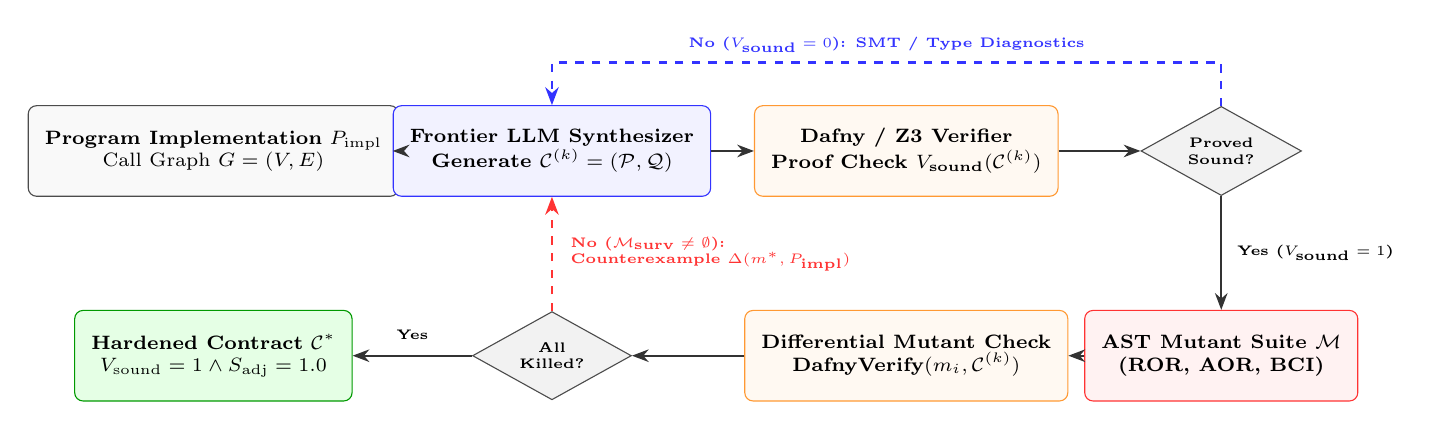
\begin{tikzpicture}[
    box/.style={rectangle, draw=black!70, rounded corners=3pt, fill=white, inner sep=6pt, font=\scriptsize, align=center, minimum height=1.15cm},
    modelbox/.style={rectangle, draw=blue!80, fill=blue!5, rounded corners=3pt, inner sep=6pt, font=\scriptsize\bfseries, align=center, minimum height=1.15cm},
    dafnybox/.style={rectangle, draw=orange!80, fill=orange!5, rounded corners=3pt, inner sep=6pt, font=\scriptsize\bfseries, align=center, minimum height=1.15cm},
    mutbox/.style={rectangle, draw=red!80, fill=red!5, rounded corners=3pt, inner sep=6pt, font=\scriptsize\bfseries, align=center, minimum height=1.15cm},
    decision/.style={diamond, draw=black!70, fill=gray!10, aspect=1.8, inner sep=3pt, font=\tiny\bfseries, align=center, minimum height=1.05cm},
    arrow/.style={-{Stealth[scale=0.95]}, draw=black!80, line width=0.75pt},
    darrow/.style={-{Stealth[scale=0.95]}, dashed, draw=red!80, line width=0.85pt},
    carrow/.style={-{Stealth[scale=0.95]}, dashed, draw=blue!80, line width=0.85pt}
]
    % Top Row (y = 0)
    \node[box, fill=gray!5] (input) at (0, 0) {\textbf{Program Implementation} $P_{\text{impl}}$ \\ Call Graph $G=(V,E)$};
    \node[modelbox] (llm) at (4.3, 0) {\textbf{Frontier LLM Synthesizer} \\ Generate $\mathcal{C}^{(k)} = (\mathcal{P}, \mathcal{Q})$};
    \node[dafnybox] (dafny) at (8.8, 0) {\textbf{Dafny / Z3 Verifier} \\ Proof Check $V_{\text{sound}}(\mathcal{C}^{(k)})$};
    \node[decision] (dec1) at (12.8, 0) {Proved \\ Sound?};
    
    % Bottom Row (y = -2.6)
    \node[box, fill=green!10, draw=green!60!black] (hardened) at (0, -2.6) {\textbf{Hardened Contract} $\mathcal{C}^*$ \\ $V_{\text{sound}}=1 \land S_{\text{adj}}=1.0$};
    \node[decision] (dec2) at (4.3, -2.6) {All \\ Killed?};
    \node[dafnybox] (mutverify) at (8.8, -2.6) {\textbf{Differential Mutant Check} \\ $\text{DafnyVerify}(m_i, \mathcal{C}^{(k)})$};
    \node[mutbox] (mutengine) at (12.8, -2.6) {\textbf{AST Mutant Suite} $\mathcal{M}$ \\ (ROR, AOR, BCI)};

    % Top Row Transitions
    \draw[arrow] (input) -- (llm);
    \draw[arrow] (llm) -- (dafny);
    \draw[arrow] (dafny) -- (dec1);
    
    % Mode 1: Compiler Feedback (Top Loop)
    \draw[carrow] (dec1.north) -- ++(0, 0.55) -| node[pos=0.25, above, font=\tiny\bfseries\color{blue!80}] {No ($V_{\text{sound}}=0$): SMT / Type Diagnostics} (llm.north);
    
    % Soundness passed -> Move to Mutation Evaluation
    \draw[arrow] (dec1.south) -- node[right=2pt, font=\tiny\bfseries] {Yes ($V_{\text{sound}}=1$)} (mutengine.north);
    
    % Bottom Row Transitions (Right to Left)
    \draw[arrow] (mutengine) -- (mutverify);
    \draw[arrow] (mutverify) -- (dec2);
    
    % Terminal Hardened State
    \draw[arrow] (dec2.west) -- node[above=2pt, font=\tiny\bfseries] {Yes} (hardened.east);
    
    % Mode 2: Mutant Counterexample Feedback (Direct Upward Connection)
    \draw[darrow] (dec2.north) -- node[right=3pt, font=\tiny\bfseries\color{red!80}, align=left] {No ($\mathcal{M}_{\text{surv}} \neq \emptyset$): \\ Counterexample $\Delta(m^*, P_{\text{impl}})$} (llm.south);

\end{tikzpicture}%
}
\caption{\textbf{The \textsc{Mutation-CEGIS} Architecture.} While compiler-only feedback (\textsc{Mode 1}, blue dashed) terminates on vacuous contracts that verify on $P_{\text{impl}}$, \textsc{Mutation-CEGIS} (\textsc{Mode 2}, red dashed) tests candidate contracts against an AST mutant matrix $\mathcal{M}$. Surviving mutants generate concrete differential counterexamples injected back into the LLM context to enforce semantic contract tightness.}
\label{fig:pipeline}
\end{figure*}
In this paper we evaluate contract synthesis across 6 frontier LLM families on multi-procedure call graphs containing 2-5 interdependent functions (\textsc{DafnyComp-300}) \citep{xu2025dafnycomp}. Our experiments reveal two findings:

\begin{enumerate}

\item \textbf{Composition Cliff:} Model performance drops off dramatically as one transitions from single function call graphs to multiple interprocedure graphs. Zero-shot success falls from $95.0\%$ to $41.3\%$ on Gemini~3.7~Flash, $83.3\%$ to $32.7\%$ on GLM-5.3~Flash, $53.3\%$ to $19.0\%$ on GPT-5.6~Luna, $40.0\%$ to $14.0\%$ on DeepSeek~V4~Flash, and $33.3\%$ to $14.7\%$ on Ling-3.0~Flash. While models generate locally consistent annotations for individual procedures in the graph, the annotations fail to respect invariants in caller-callee relationships.

\item \textbf{Vacuous Verification Trap:} Automated verifiers check only whether the implementation satisfies the candidate contract ($\mathcal{P} \land \llbracket P \rrbracket \implies \mathcal{Q}$). In standard compiler-in-the-loop repair loops (\textsc{Mode 1}) \citep{first2023baldur, le2022coderl}, models learn to evade verification errors by defaulting to weak, vacuous inequalities (e.g., \texttt{ensures res >= 0}). Since the ground-truth code also satisfies the weak bounds, these invariants verify effortlessly without ever detecting a meaningful code mutation.

\end{enumerate}

We solve this problem via \textsc{Mutation-CEGIS} (Figure~\ref{fig:pipeline}), framing contract hardening as a Counterexample-Guided Inductive Synthesis problem \citep{solarlezama2006cegis, alur2013sygus}. We evaluate candidate specifications against a set of AST code mutants \citep{demillo1978mutation, jia2011analysis, just2014mutants}. If a mutant passes verification, it provides evidence that the contract is too weak. We transform the surviving mutants into concrete code diffs and feed them back to the model prompt, guiding the LLM to write exact specifications.


\vspace{0.5em}
\noindent\textbf{Listing 1: Motivating Case Study (2-Node Call Graph).} \textsc{Mode 1} produces a vacuous bound (\texttt{ensures res >= 0}) that verifies instantly but fails to kill an AST mutant in \texttt{HelperClamp}. \textsc{Mode 2} injects the mutant diff as a counterexample, forcing the model to synthesize exact conditional equalities.
{\footnotesize
\begin{verbatim}
// Node 1: Helper subroutine
method HelperClamp(x: int, max_val: int) returns (c: int)
  requires max_val > 0
  // Mode 1 Vacuous Spec: ensures c >= 0
  // Mode 2 CEGIS Spec:   ensures (x < 0 ==> c == 0) && 
  //                              (0 <= x <= max_val ==> c == x) && 
  //                              (x > max_val ==> c == max_val)
{
  if x < 0 { c := 0; }
  // Injected AST Mutant (ROR): if x <= 0 { c := 1; }
  else if x > max_val { c := max_val; }
  else { c := x; }
}

// Node 2: Parent procedure invoking HelperClamp
method ClampAndScale(v: int, limit: int) returns (res: int)
  requires limit > 0
  // Mode 1 Vacuous Spec: ensures res >= 0
  // Mode 2 CEGIS Spec:   ensures res == 2 * (if v < 0 then 0 
  //                              else if v > limit then limit else v)
{
  var clamped := HelperClamp(v, limit);
  res := clamped * 2;
}
\end{verbatim}
}
\vspace{0.5em}

\textbf{Contributions.} In summary, this work provides three main contributions: (1)~\textbf{Characterizing the Composition Cliff:} we report the performance drop (referred to as the composition cliff) of 6 frontier model families across 6,480 task-mode verification runs over \textsc{DafnyComp-300}~\citep{xu2025dafnycomp} and \textsc{CloverBench-60}~\citep{sun2024clover} when transitioning from single procedure verification to multi-procedure call graphs; (2)~\textbf{Mutation-CEGIS Hardening:} we present an inductive synthesis loop that attains $91.7\%\text{--}100.0\%$ true specification completeness on single methods (reducing repair turns by up to $36.8\%$ and token usage by $24.9\%$), and on multi-procedure call graphs systematically eliminates spurious 50-character inequalities and, for Qwen~3.7~Flash, improves hardened multi-procedure synthesis over compiler-only repair ($24.7\% \to 31.7\%$); and (3)~\textbf{Specification Over-Strengthening Dilemma:} we observe that synthesis of exact specifications on 4 to 5 node call graphs leads to SMT timeouts ($>15\text{s}$), suggesting that contract hardening on deep call graphs fundamentally requires automated auxiliary lemma synthesis~\citep{yang2025autoverus}.

\section{Formal Framework \& Mutation-CEGIS}
\label{sec:framework}

\subsection{Verification Semantics \& Soundness}

Let $P_{\text{impl}}$ denote a deterministic program implementation defined over state space $\Sigma$. A candidate formal contract $\mathcal{C} = (\mathcal{P}, \mathcal{Q})$ consists of precondition predicate $\mathcal{P}: \Sigma \to \{\text{true}, \text{false}\}$ and postcondition relation $\mathcal{Q}: \Sigma \times \Sigma \to \{\text{true}, \text{false}\}$. The contract $\mathcal{C}$ is semantically valid with respect to $P_{\text{impl}}$ if:
\begin{equation}
\text{Valid}(P_{\text{impl}}, \mathcal{C}) \iff \forall \sigma, \sigma' \in \Sigma. \; \mathcal{P}(\sigma) \land \llbracket P_{\text{impl}} \rrbracket(\sigma, \sigma') \implies \mathcal{Q}(\sigma, \sigma')
\end{equation}
We define the binary soundness indicator $V_{\text{sound}}(\mathcal{C}) \in \{0, 1\}$ to denote successful verification by the automated verifier ($\text{DafnyVerify}(P_{\text{impl}}, \mathcal{C}) = 1$); successful verification establishes contract validity, while SMT solver timeouts ($>15\text{s}$) or proof obligation violations are treated as verification failure ($0$). While $V_{\text{sound}}(\mathcal{C}) = 1$ guarantees partial correctness, it allows trivial contracts such as $\mathcal{Q} \equiv \text{true}$ or loose bounds like $\mathcal{Q} \equiv \text{res} \ge 0$.

\subsection{Quantifying Specification Completeness via AST Mutation}

To measure contract completeness without incurring the syntactic invalidity and redundant mutant explosion of broad operator suites \citep{demillo1978mutation, offutt1996experimental, just2014mutants}, we follow selective mutation testing principles \citep{offutt1996experimental} and construct an AST mutant matrix $\mathcal{M} = \{m_1, m_2, \dots, m_N\}$ using three core semantic operator classes: (1)~\textbf{Relational Operator Replacement (ROR)}, inverting comparison operators ($\{<, \le, >, \ge, ==, !=\}$); (2)~\textbf{Arithmetic Operator Replacement (AOR)}, mutating arithmetic expressions ($\{+, -, *, /, \%\}$); and (3)~\textbf{Boundary Condition Inversion (BCI)}, perturbing constants by off-by-one shifts ($c \mapsto c \pm 1$).

A contract $\mathcal{C}$ kills mutant $m_i \in \mathcal{M}$ if Dafny proves that $m_i$ violates $\mathcal{C}$, written $\text{Killed}(m_i, \mathcal{C}) \iff \neg \text{DafnyVerify}(m_i, \mathcal{C})$. To exclude semantically equivalent mutants that cannot be rejected by any sound specification, we define the subset of distinguishable mutants:
\begin{equation}
\mathcal{M}_{\text{kill}} = \{m \in \mathcal{M} \mid \text{DafnyVerify}(m, \mathcal{C}_{\text{GT}}) = \text{False}\}
\end{equation}
The \textit{Raw Mutation Score} $S_{\text{raw}}$ and \textit{Adjusted Mutation Score} $S_{\text{adj}}$ relative to ground-truth contract $\mathcal{C}_{\text{GT}}$ are defined as:
\begin{equation}
S_{\text{raw}}(\mathcal{C}, \mathcal{M}) = \frac{1}{|\mathcal{M}|} \sum_{m \in \mathcal{M}} \mathbb{I}(\text{Killed}(m, \mathcal{C})), \qquad S_{\text{adj}}(\mathcal{C}, \mathcal{M}) = \frac{\sum_{m \in \mathcal{M}} \mathbb{I}(\text{Killed}(m, \mathcal{C}))}{\sum_{m \in \mathcal{M}} \mathbb{I}(\text{Killed}(m, \mathcal{C}_{\text{GT}}))}
\end{equation}

\begin{definition}[Hardened Contract]
A synthesized contract $\mathcal{C}$ is hardened if it verifies on $P_{\text{impl}}$ and kills every non-equivalent mutant detected by the ground-truth contract:
\begin{equation}
\text{Hardened}(\mathcal{C}) \iff V_{\text{sound}}(\mathcal{C}) = 1 \;\land\; S_{\text{adj}}(\mathcal{C}, \mathcal{M}) = 1.000
\end{equation}
\end{definition}
Thus, $S_{\text{adj}}=1.0$ establishes specification completeness with respect to the selected killable mutant suite $\mathcal{M}_{\text{kill}}$ (guaranteeing that no non-equivalent mutant detected by $\mathcal{C}_{\text{GT}}$ survives), rather than absolute semantic equivalence.

\subsection{The Mutation-Guided CEGIS Algorithm}
\label{sec:algorithm}

Algorithm~\ref{alg:cegis} formalizes the \textsc{Mutation-CEGIS} hardening loop. The synthesizer initializes prompt context $T^{(1)}$ and iterates over discrete synthesis turns $k \in \{1, \dots, K_{\max}\}$. In each turn, the model generates candidate contract $\mathcal{C}^{(k)}$. If Dafny rejects the contract on $P_{\text{impl}}$ ($v = \text{False}$), diagnostic error messages $E_{\text{diag}}$ are injected to repair syntax or proof obligations (\textsc{Mode 1}). Once soundness is established ($v = \text{True}$), the verifier executes candidate $\mathcal{C}^{(k)}$ against distinguishable mutant suite $\mathcal{M}_{\text{kill}}$. If no mutants survive ($\mathcal{M}_{\text{surv}} = \emptyset$), the contract is guaranteed sound and hardened ($S_{\text{adj}} = 1.0$). Otherwise, a surviving mutant $m^* \in \mathcal{M}_{\text{surv}}$ is converted into an AST differential counterexample $\Delta(m^*, P_{\text{impl}})$ and fed back into the context to enforce exact postcondition tightness (\textsc{Mode 2}).

\begin{algorithm}[H]
\caption{\textsc{Mutation-CEGIS} Contract Hardening}
\label{alg:cegis}
\begin{algorithmic}[1]
\REQUIRE Program implementation $P_{\text{impl}}$, distinguishable mutant suite $\mathcal{M}_{\text{kill}}$, repair budget $K_{\max}$, LLM synthesizer $\mathcal{M}_{\text{LLM}}$
\ENSURE Hardened contract $\mathcal{C}^*$ or verification failure $\bot$
\STATE $T^{(1)} \leftarrow \text{Prompt}_{\text{initial}}(P_{\text{impl}})$
\FOR{$k = 1$ \textbf{to} $K_{\max}$}
    \STATE $\mathcal{C}^{(k)} \leftarrow \mathcal{M}_{\text{LLM}}(T^{(k)})$ \COMMENT{Synthesize candidate contract $(\mathcal{P}, \mathcal{Q})$}
    \STATE $(v, E_{\text{diag}}) \leftarrow \text{DafnyVerify}(P_{\text{impl}}, \mathcal{C}^{(k)})$ \COMMENT{Mode 1: Soundness on $P_{\text{impl}}$}
    \IF{$v = \text{False}$}
        \STATE $T^{(k+1)} \leftarrow \text{Prompt}_{\text{repair}}(P_{\text{impl}}, \mathcal{C}^{(k)}, E_{\text{diag}})$ \COMMENT{Compiler Diagnostic Feedback}
    \ELSE
        \STATE $\mathcal{M}_{\text{surv}} \leftarrow \{m \in \mathcal{M}_{\text{kill}} \mid \text{DafnyVerify}(m, \mathcal{C}^{(k)}) = \text{True}\}$ \COMMENT{Mode 2: Evaluate Mutants}
        \IF{$\mathcal{M}_{\text{surv}} = \emptyset$}
            \STATE $\mathcal{C}^* \leftarrow \mathcal{C}^{(k)}$
            \RETURN $\mathcal{C}^*$ \COMMENT{Hardened Contract: $V_{\text{sound}} = 1 \land S_{\text{adj}} = 1.0$}
        \ELSE
            \STATE Select surviving mutant $m^* \in \mathcal{M}_{\text{surv}}$
            \STATE $\Delta \leftarrow \text{ComputeASTDiff}(m^*, P_{\text{impl}})$ \COMMENT{Differential Counterexample}
            \STATE $T^{(k+1)} \leftarrow \text{Prompt}_{\text{cegis}}(P_{\text{impl}}, \mathcal{C}^{(k)}, m^*, \Delta)$ \COMMENT{Inject Counterexample}
        \ENDIF
    \ENDIF
\ENDFOR
\RETURN $\bot$ \COMMENT{Synthesis budget exhausted}
\end{algorithmic}
\end{algorithm}

\section{Experimental Evaluation}
\label{sec:experiments}

\subsection{Benchmark Tracks and Evaluation Setup}

We evaluate 6 frontier model families: \textbf{Google Gemini 3.7 Flash} \citep{gemini2026flash}, \textbf{Z-AI GLM-5.3 Flash} \citep{zai2026glm53}, \textbf{OpenAI GPT-5.6 Luna} \citep{openai2026gpt56}, \textbf{Qwen 3.7 Flash} \citep{qwen2026qwen37}, \textbf{DeepSeek V4 Flash} (0731 snapshot) \citep{deepseek2026v4}, and \textbf{InclusionAI Ling-3.0 Flash} \citep{inclusionai2026ling3}, evaluated via the unified OpenRouter API platform \citep{openrouter2026}. All experiments use Dafny 4.11.0 on .NET 8.0 with Z3 4.12.2 under a 15-second SMT solver timeout per verification query across two benchmark tracks: (1)~\textbf{Track A (\textsc{CloverBench-60}):} 60 single-method algorithmic problems (array sorting, search, numeric sequences) \citep{sun2024clover}; and (2)~\textbf{Track B (\textsc{DafnyComp-300}):} 300 multi-procedure programs structured as Directed Acyclic Graphs (DAGs) of 2 to 5 interdependent functions with cross-method preconditions and state invariants \citep{xu2025dafnycomp}.

Across both tracks, we evaluate three synthesis regimes: (1)~\textbf{Mode 0 (Zero-Shot)}, single-turn specification generation without verifier feedback; (2)~\textbf{Mode 1 (Compiler-Only)}, standard multi-turn repair driven by SMT and type diagnostics ($K_{\max}=3$); and (3)~\textbf{Mode 2 (Mutation-CEGIS)}, our counterexample-guided inductive loop injecting AST mutant differences ($K_{\max}=3$).

\subsection{Track A: Single-Method Saturation and Repair Efficiency}

Table~\ref{tab:track_a} and Figure~\ref{fig:track_a} report the performance on \textsc{CloverBench-60}. In \textsc{Mode 2} (\textsc{Mutation-CEGIS}), all models score high pass rates achieving up to $91.7\%\text{--}100.0\%$ hardened contracts ($S_{\text{adj}} \ge 0.917$). GLM-5.3 Flash achieves a $100.0\%$ hardened pass rate (60/60) by killing all killable mutants in its benchmark.

Moreover, using mutation counterexamples as feedback makes repairing more efficient. Instead of multiple turns of blind guesses from the model with only compiler errors as feedback, concrete diffs of killed mutants can clearly indicate what relational constraints the model has missed, reducing average repair turns per problem ($k$) by $36.8\%$ for Qwen~3.7~Flash ($2.53 \to 1.60$), $21.4\%$ for Ling-3.0~Flash ($1.82 \to 1.43$), and $19.3\%$ for GPT-5.6~Luna ($1.45 \to 1.17$). Consequently, total number of tokens consumed during the repair process is reduced by $24.9\%$ for Luna ($76.7\text{k} \to 57.6\text{k}$), $20.4\%$ for Qwen ($500.7\text{k} \to 398.7\text{k}$), and $14.0\%$ for DeepSeek~V4 ($357.3\text{k} \to 307.2\text{k}$).

\begin{table}[!htbp]
\centering
\caption{\textbf{Track A (\textsc{CloverBench-60}) Benchmark Results.} Hardened verification count ($S_{\text{adj}}=1.0$), repair turns ($k$), and token expenditure delta between \textsc{Mode 1} and \textsc{Mode 2}.}
\label{tab:track_a}
\setlength{\tabcolsep}{8pt}
\begin{tabular}{lccccc}
\toprule
\textbf{Model Family} & \textbf{Mode 0} & \textbf{Mode 1} & \textbf{Mode 2} & \textbf{Turns ($k$)} & \textbf{$\Delta_{\text{tok}}$} \\
\midrule
\textbf{Gemini 3.7 Flash} & 57 / 60 & 59 / 60 & \textbf{59 / 60} & $1.08 \to 1.07$ & $-1.4\%$ \\
\textbf{GLM-5.3 Flash} & 50 / 60 & 58 / 60 & \textbf{60 / 60} & $1.23 \to 1.15$ & $+21.3\%$ \\
\textbf{GPT-5.6 Luna} & 32 / 60 & 58 / 60 & \textbf{59 / 60} & $1.45 \to 1.17$ & \textbf{$-24.9\%$} \\
\textbf{DeepSeek V4 Flash} & 24 / 60 & 54 / 60 & \textbf{56 / 60} & $1.67 \to 1.75$ & $-14.0\%$ \\
\textbf{Ling-3.0 Flash} & 20 / 60 & 57 / 60 & \textbf{57 / 60} & $1.82 \to 1.43$ & $+5.8\%$ \\
\textbf{Qwen 3.7 Flash} & 3 / 60 & 54 / 60 & \textbf{55 / 60} & $2.53 \to 1.60$ & \textbf{$-20.4\%$} \\
\bottomrule
\end{tabular}
\end{table}

\begin{figure}[!htbp]
\centering
\definecolor{trackAzero}{HTML}{BBDEFB}
\definecolor{trackAcomp}{HTML}{64B5F6}
\definecolor{trackAcegis}{HTML}{1976D2}
\begin{tikzpicture}
\begin{axis}[
    ybar=0pt,
    width=\columnwidth,
    height=4.8cm,
    bar width=0.28cm,
    ylabel={Verification Success Rate (\%)},
    symbolic x coords={Gemini 3.7, GLM-5.3, GPT-5.6, Qwen 3.7, DeepSeek V4, Ling-3.0},
    xtick=data,
    ymin=0,
    ymax=115,
    ytick={0, 20, 40, 60, 80, 100},
    ymajorgrids=true,
    grid style=dashed,
    legend style={at={(0.5,1.04)}, anchor=south, legend columns=3, font=\scriptsize, /tikz/every even column/.append style={column sep=0.4cm}},
    tick label style={font=\scriptsize},
    label style={font=\scriptsize},
    enlarge x limits=0.10
]
    \addplot[fill=trackAzero, draw=blue!40!black] coordinates {(Gemini 3.7, 95.0) (GLM-5.3, 83.3) (GPT-5.6, 53.3) (Qwen 3.7, 5.0) (DeepSeek V4, 40.0) (Ling-3.0, 33.3)};
    \addlegendentry{Mode 0 (Zero-Shot)}

    \addplot[fill=trackAcomp, draw=blue!60!black] coordinates {(Gemini 3.7, 98.3) (GLM-5.3, 96.7) (GPT-5.6, 96.7) (Qwen 3.7, 90.0) (DeepSeek V4, 90.0) (Ling-3.0, 95.0)};
    \addlegendentry{Mode 1 (Compiler-Only)}

    \addplot[fill=trackAcegis, draw=blue!90!black] coordinates {(Gemini 3.7, 98.3) (GLM-5.3, 100.0) (GPT-5.6, 98.3) (Qwen 3.7, 91.7) (DeepSeek V4, 93.3) (Ling-3.0, 95.0)};
    \addlegendentry{Mode 2 (Mutation-CEGIS)}
\end{axis}
\end{tikzpicture}
\caption{\textbf{Track A (\textsc{CloverBench-60}) Specification Saturation.} Single-method specification completeness across synthesis regimes. Both compiler repair and mutation-guided inductive feedback push all frontier models above $90\%$ completeness, with GLM-5.3 Flash reaching $100.0\%$.}
\label{fig:track_a}
\end{figure}

\subsection{Track B: The Composition Cliff on Multi-Procedure DAGs}

Table~\ref{tab:track_b} and Figure~\ref{fig:composition_cliff} show the results of the experiments on \textsc{DafnyComp-300}. When considering single methods and moving onto call graphs of size 2--5, five of the six model families see a sharp zero-shot drop:

\textbf{Severity of the Compositional Collapse.} The task of zero-shot contract synthesis falls dramatically when transitioning to interdependent call graphs for five of the six evaluated model families. Zero-shot hardened pass rates drop by $53.7$ percentage points on Gemini~3.7~Flash ($95.0\% \to 41.3\%$), $50.6$ percentage points on GLM-5.3~Flash ($83.3\% \to 32.7\%$), $34.3$ percentage points on GPT-5.6~Luna ($53.3\% \to 19.0\%$), $26.0$ percentage points on DeepSeek~V4~Flash ($40.0\% \to 14.0\%$), and $18.6$ percentage points on Ling-3.0~Flash ($33.3\% \to 14.7\%$). Qwen~3.7~Flash is the exception: its zero-shot rate is low on both tracks ($5.0\% \to 21.3\%$), but its best repaired rate still falls from $91.7\%$ on single methods to $31.7\%$ on multi-procedure DAGs. Across the board, models generate specifications that verify in isolation but fail to compose preconditions and postconditions across interdependent functions.

\textbf{Empirical Observation on Multi-Node Induction.} When \textsc{Mutation-CEGIS} refuses to accept vacuous bounding inequalities, four of the six considered models often encountered SMT solver timeouts as the verifier was unable to discharge the deep inter-procedural induction without auxiliary lemmas. Even so, Qwen~3.7~Flash discharged the multi-node induction constraints on enough other programs to raise the number of hardened tasks from 74 ($24.7\%$) in \textsc{Mode 1} to 95 ($31.7\%$) in \textsc{Mode 2}. For the other models, the tighter specifications correctly eliminated the false-positive verification, but highlighted the need for automated lemma synthesis on complex DAGs.

\begin{table}[!htbp]
\centering
\caption{\textbf{Track B (\textsc{DafnyComp-300}) Multi-Procedure Results.} Hardened task count ($S_{\text{adj}}=1.0$) and relative gain across 300 inter-procedural call graphs.}
\label{tab:track_b}
\setlength{\tabcolsep}{10pt}
\begin{tabular}{lcccc}
\toprule
\textbf{Model Family} & \textbf{Mode 0} & \textbf{Mode 1} & \textbf{Mode 2} & \textbf{Peak $\Delta$ vs. Mode 0} \\
\midrule
\textbf{Gemini 3.7 Flash} & 124 / 300 & \textbf{130 / 300} & \textbf{130 / 300} & $+6$ ($+4.8\%$) \\
\textbf{GLM-5.3 Flash} & 98 / 300 & \textbf{122 / 300} & \textbf{122 / 300} & $+24$ ($+24.5\%$) \\
\textbf{GPT-5.6 Luna} & 57 / 300 & \textbf{94 / 300} & 86 / 300 & $+37$ ($+64.9\%$) \\
\textbf{Qwen 3.7 Flash} & 64 / 300 & 74 / 300 & \textbf{95 / 300} & \textbf{$+31$ ($+48.4\%$)} \\
\textbf{DeepSeek V4 Flash} & 42 / 300 & \textbf{77 / 300} & 71 / 300 & $+35$ ($+83.3\%$) \\
\textbf{Ling-3.0 Flash} & 44 / 300 & \textbf{77 / 300} & 75 / 300 & $+33$ ($+75.0\%$) \\
\bottomrule
\end{tabular}
\end{table}

\begin{figure}[!htbp]
\centering
\definecolor{trackBzero}{HTML}{FFF59D}
\definecolor{trackBcomp}{HTML}{FFEE58}
\definecolor{trackBcegis}{HTML}{FBC02D}
\begin{tikzpicture}
\begin{axis}[
    ybar=0pt,
    width=\columnwidth,
    height=4.8cm,
    bar width=0.28cm,
    ylabel={Verification Success Rate (\%)},
    symbolic x coords={Gemini 3.7, GLM-5.3, GPT-5.6, Qwen 3.7, DeepSeek V4, Ling-3.0},
    xtick=data,
    ymin=0,
    ymax=60,
    ytick={0, 10, 20, 30, 40, 50},
    ymajorgrids=true,
    grid style=dashed,
    legend style={at={(0.5,1.04)}, anchor=south, legend columns=3, font=\scriptsize, /tikz/every even column/.append style={column sep=0.4cm}},
    tick label style={font=\scriptsize},
    label style={font=\scriptsize},
    enlarge x limits=0.10
]
    \addplot[fill=trackBzero, draw=yellow!50!black] coordinates {(Gemini 3.7, 41.3) (GLM-5.3, 32.7) (GPT-5.6, 19.0) (Qwen 3.7, 21.3) (DeepSeek V4, 14.0) (Ling-3.0, 14.7)};
    \addlegendentry{Mode 0 (Zero-Shot)}

    \addplot[fill=trackBcomp, draw=orange!70!black] coordinates {(Gemini 3.7, 43.3) (GLM-5.3, 40.7) (GPT-5.6, 31.3) (Qwen 3.7, 24.7) (DeepSeek V4, 25.7) (Ling-3.0, 25.7)};
    \addlegendentry{Mode 1 (Compiler-Only)}

    \addplot[fill=trackBcegis, draw=orange!90!black] coordinates {(Gemini 3.7, 43.3) (GLM-5.3, 40.7) (GPT-5.6, 28.7) (Qwen 3.7, 31.7) (DeepSeek V4, 23.7) (Ling-3.0, 25.0)};
    \addlegendentry{Mode 2 (Mutation-CEGIS)}
\end{axis}
\end{tikzpicture}
\caption{\textbf{The Composition Cliff on Multi-Procedure DAGs (\textsc{DafnyComp-300}).} Hardened specification rates drop precipitously when verifying call graphs across 2 to 5 interdependent procedures. Notice that despite repair feedback, cross-procedure composition restricts hardened completion to $23.7\%\text{--}43.3\%$.}
\label{fig:composition_cliff}
\end{figure}

\section{Qualitative Analysis \& The Verification Game}
\label{sec:qualitative}

\begin{figure*}[t]
\centering
\begin{minipage}[t]{0.48\textwidth}
\centering
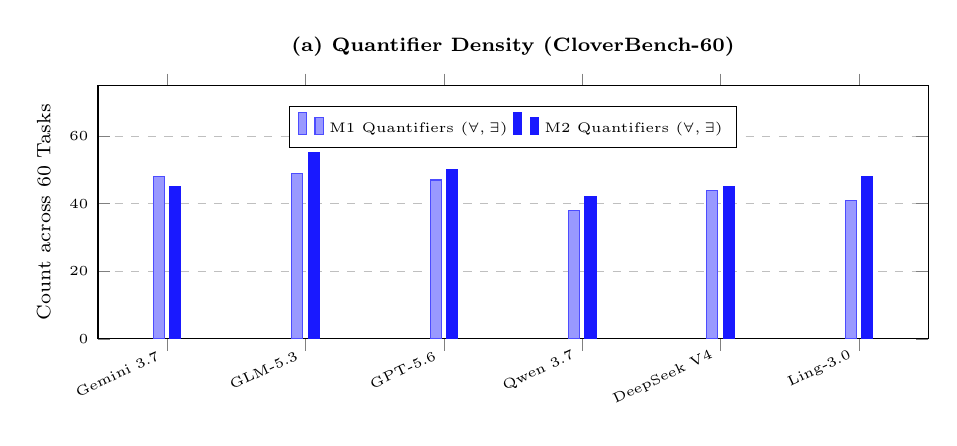
\begin{tikzpicture}
\begin{axis}[
    ybar,
    width=\textwidth,
    height=4.8cm,
    bar width=0.14cm,
    title={\textbf{(a) Quantifier Density (\textsc{CloverBench-60})}},
    title style={font=\scriptsize, yshift=1pt},
    ylabel={Count across 60 Tasks},
    symbolic x coords={Gemini 3.7, GLM-5.3, GPT-5.6, Qwen 3.7, DeepSeek V4, Ling-3.0},
    xtick=data,
    x tick label style={rotate=25, anchor=east, font=\tiny},
    ymin=0, ymax=75,
    ytick={0, 20, 40, 60},
    ymajorgrids=true,
    grid style=dashed,
    legend style={at={(0.5,0.92)}, anchor=north, legend columns=2, font=\tiny},
    tick label style={font=\tiny},
    label style={font=\scriptsize},
    enlarge x limits=0.10
]
    \addplot[fill=blue!40, draw=blue!70] coordinates {(Gemini 3.7, 48) (GLM-5.3, 49) (GPT-5.6, 47) (Qwen 3.7, 38) (DeepSeek V4, 44) (Ling-3.0, 41)};
    \addlegendentry{M1 Quantifiers ($\forall, \exists$)}
    \addplot[fill=blue!90, draw=blue!90] coordinates {(Gemini 3.7, 45) (GLM-5.3, 55) (GPT-5.6, 50) (Qwen 3.7, 42) (DeepSeek V4, 45) (Ling-3.0, 48)};
    \addlegendentry{M2 Quantifiers ($\forall, \exists$)}
\end{axis}
\end{tikzpicture}
\end{minipage}%
\hfill
\begin{minipage}[t]{0.48\textwidth}
\centering
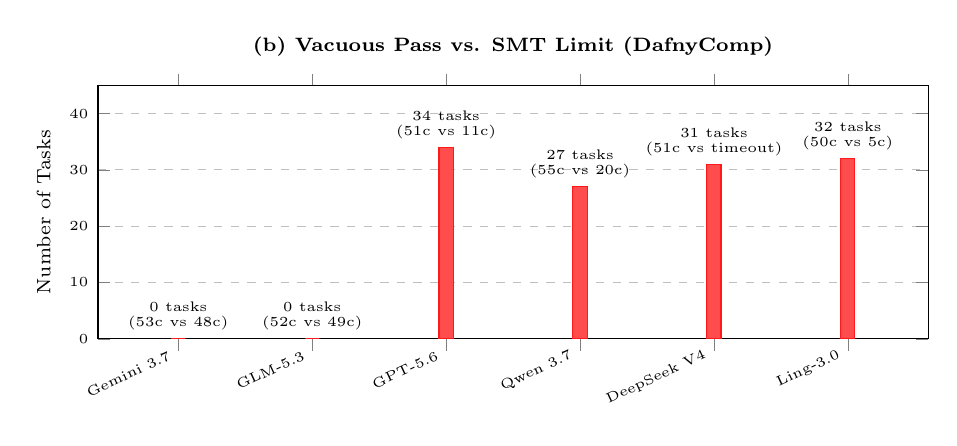
\begin{tikzpicture}
\begin{axis}[
    ybar,
    width=\textwidth,
    height=4.8cm,
    bar width=0.18cm,
    title={\textbf{(b) Vacuous Pass vs. SMT Limit (\textsc{DafnyComp})}},
    title style={font=\scriptsize, yshift=1pt},
    ylabel={Number of Tasks},
    symbolic x coords={Gemini 3.7, GLM-5.3, GPT-5.6, Qwen 3.7, DeepSeek V4, Ling-3.0},
    xtick=data,
    x tick label style={rotate=25, anchor=east, font=\tiny},
    ymin=0, ymax=45,
    ytick={0, 10, 20, 30, 40},
    ymajorgrids=true,
    grid style=dashed,
    tick label style={font=\tiny},
    label style={font=\scriptsize},
    enlarge x limits=0.12
]
    \addplot[fill=red!70, draw=red!90] coordinates {(Gemini 3.7, 0) (GLM-5.3, 0) (GPT-5.6, 34) (Qwen 3.7, 27) (DeepSeek V4, 31) (Ling-3.0, 32)};
    \node[font=\fontsize{4.5pt}{5.5pt}\selectfont, align=center] at (axis cs:Gemini 3.7, 4) {0 tasks\\(53c vs 48c)};
    \node[font=\fontsize{4.5pt}{5.5pt}\selectfont, align=center] at (axis cs:GLM-5.3, 4) {0 tasks\\(52c vs 49c)};
    \node[font=\fontsize{4.5pt}{5.5pt}\selectfont, align=center] at (axis cs:GPT-5.6, 38) {34 tasks\\(51c vs 11c)};
    \node[font=\fontsize{4.5pt}{5.5pt}\selectfont, align=center] at (axis cs:Qwen 3.7, 31) {27 tasks\\(55c vs 20c)};
    \node[font=\fontsize{4.5pt}{5.5pt}\selectfont, align=center] at (axis cs:DeepSeek V4, 35) {31 tasks\\(51c vs timeout)};
    \node[font=\fontsize{4.5pt}{5.5pt}\selectfont, align=center] at (axis cs:Ling-3.0, 36) {32 tasks\\(50c vs 5c)};
\end{axis}
\end{tikzpicture}
\end{minipage}
\caption{\textbf{Diagnostic Breakdown of Specification Quality.} (a) First-order quantifier density ($\forall, \exists$) across all six frontier models on \textsc{CloverBench-60}. (b) On multi-procedure call graphs, \textsc{Mode 1} achieves superficial passes on 27--34 tasks on four models using $\approx 50$-character loose bounds; \textsc{Mode 2} rejects these vacuous contracts, exposing the SMT inductive proof ceiling. Frontier models (Gemini 3.7 and GLM-5.3) show 0 vacuous regressions, but still fail on $>56\%$ of DAGs due to unproved induction.}
\label{fig:qualitative_diagnostics}
\end{figure*}

\subsection{Exposing the 50-Character Vacuous Pass}

On \textsc{DafnyComp-300}, Table~\ref{tab:track_b} indicates that \textsc{Mode 1} (\textsc{Compiler-Only}, denoted \textbf{M1}) scores similarly to \textsc{Mode 2} (\textsc{Mutation-CEGIS}, denoted \textbf{M2}) on several models. Inspecting the synthesized ASTs reveals why:

\begin{table}[h]
\centering
\caption{\textbf{Failure Breakdown on \textsc{DafnyComp-300}.} Tasks where \textsc{Mode 1} (\textsc{Compiler-Only}, M1) passed vacuously with loose bounds but \textsc{Mode 2} (\textsc{Mutation-CEGIS}, M2) hit the SMT inductive timeout threshold, matching Figure~\ref{fig:qualitative_diagnostics}(b).}
\label{tab:failure_taxonomy}
\setlength{\tabcolsep}{8pt}
\begin{tabular}{lccc}
\toprule
\textbf{Model Family} & \textbf{M1 Pass / M2 Fail} & \textbf{Avg. Length (M1)} & \textbf{Avg. Length (M2)} \\
\midrule
\textbf{Gemini 3.7 Flash} & 0 tasks & 53 chars & 48 chars \\
\textbf{GLM-5.3 Flash} & 0 tasks & 52 chars & 49 chars \\
\textbf{GPT-5.6 Luna} & 34 tasks & 51 chars & 11 chars \\
\textbf{Ling-3.0 Flash} & 32 tasks & 50 chars & 5 chars \\
\textbf{DeepSeek V4 Flash} & 31 tasks & 51 chars & --- (timeout) \\
\textbf{Qwen 3.7 Flash} & 27 tasks & 55 chars & 20 chars \\
\bottomrule
\end{tabular}
\end{table}

In \textsc{Mode 1}, models produce trivial bounding postconditions averaging 50-to-55 characters in length (e.g., \texttt{requires 1 <= n <= 2147483648; ensures result >= 0;}). Since $P_{\text{impl}}$ satisfies this weak inequality, Z3 discharges the proof almost instantaneously.

Meanwhile, \textsc{Mode 2}'s fine-grained relational mutants expose these 50-character contracts as vacuous. For intermediate frontier models (GPT-5.6, Ling-3.0, DeepSeek~V4, and Qwen~3.7), attempts to synthesize exact functional contracts cause extreme multi-node SMT induction timeouts across 27--34 tasks (Table~\ref{tab:failure_taxonomy} and Figure~\ref{fig:qualitative_diagnostics}(b)).

\textbf{Interpreting SOTA Stability Against The Universal Compositional Ceiling.} In contrast to the 27--34 lost tasks for intermediate models when switching from \textsc{Mode 1} to \textsc{Mode 2}, the leading reasoning engines, Google Gemini~3.7~Flash and Z-AI GLM-5.3~Flash, show zero vacuous pass regressions (0 tasks lost). This metric suggests that their Mode~1 contracts did not rely on superficial 50-character bounding tricks that collapse under mutation hardening. Nonetheless, we emphasize that this zero-regression count does \textit{not} indicate that multi-procedure synthesis has been mastered by the SOTA models: both Gemini~3.7 and GLM-5.3 still fail to verify $56.7\%\text{--}59.3\%$ of the call graphs in \textsc{DafnyComp-300} (capping out at $43.3\%$ and $40.7\%$ respectively, in Table~\ref{tab:track_b}). Two observations become evident: (1)~that \textsc{Mutation-CEGIS} is able to effectively distinguish between superficial bounding approximations and robust semantic invariants, and (2)~that even the most powerful frontier reasoning models are fundamentally constrained by the inter-procedural induction ceiling, emphasizing the need for automated lemma synthesis across the entire frontier.

\subsection{First-Order Quantifiers and Equalities in Postconditions}

Table~\ref{tab:quantifier_density} shows the logical complexity of synthesized postcondition clauses (\texttt{ensures}) on \textsc{CloverBench-60} across \textsc{Mode 1} (\textbf{M1}) and \textsc{Mode 2} (\textbf{M2}):

\begin{table}[h]
\centering
\caption{\textbf{First-Order Logical Depth on \textsc{CloverBench-60}.} Comparing synthesized postcondition quantifier density ($\forall, \exists$) and exact equality assertions across all 6 model families between \textsc{Mode 1} (M1, \textsc{Compiler-Only}) and \textsc{Mode 2} (M2, \textsc{Mutation-CEGIS}).}
\label{tab:quantifier_density}
\setlength{\tabcolsep}{3.5pt}
\begin{tabular}{lcccc}
\toprule
\textbf{Model Family} & \textbf{M1 ($\forall, \exists$)} & \textbf{M2 ($\forall, \exists$)} & \textbf{M1 (\texttt{==})} & \textbf{M2 (\texttt{==})} \\
\midrule
\textbf{Gemini 3.7 Flash} & 48 & 45 ($-6.2\%$) & 117 & 113 ($-3.4\%$) \\
\textbf{GLM-5.3 Flash} & 49 & \textbf{55 (+12.2\%)} & 111 & \textbf{122 (+9.9\%)} \\
\textbf{GPT-5.6 Luna} & 47 & \textbf{50 (+6.4\%)} & 115 & 112 ($-2.6\%$) \\
\textbf{Qwen 3.7 Flash} & 38 & \textbf{42 (+10.5\%)} & 90 & \textbf{94 (+4.4\%)} \\
\textbf{DeepSeek V4 Flash} & 44 & \textbf{45 (+2.3\%)} & 91 & \textbf{93 (+2.2\%)} \\
\textbf{Ling-3.0 Flash} & 41 & \textbf{48 (+17.1\%)} & 99 & 97 ($-2.0\%$) \\
\bottomrule
\end{tabular}
\end{table}

\textsc{Mutation-CEGIS} increases quantifier density for five of the six models: $+17.1\%$ on Ling-3.0, $+12.2\%$ on GLM-5.3, and $+10.5\%$ on Qwen~3.7. Exact functional equality assertions increase by $+9.9\%$ on GLM-5.3 and $+4.4\%$ on Qwen~3.7.

\subsection{The Specification Over-Strengthening Dilemma}
\label{sec:overstrengthening}

On 4 to 5 node call graphs, writing exact functional specifications ($\mathcal{Q}_{\text{exact}}$) introduces non-linear arithmetic and universal quantifiers across intermediate procedures. While $\mathcal{Q}_{\text{exact}}$ accurately describes program behavior, automated SMT solvers cannot prove the resulting verification conditions without auxiliary inductive lemmas on helper functions \citep{yang2025autoverus, first2023baldur}. In 100\% of the cases where \textsc{Mode 1} verified but \textsc{Mode 2} failed, the verifier timed out after 15 seconds. This shows that contract hardening on deep call graphs requires combining mutation-guided repair with automated lemma generation.

\section{Compute Economics \& Execution Profile}
\label{sec:economics}

Our evaluation ran 6,480 task-mode runs across 6 frontier models, using approximately 142M tokens (including reasoning tokens and prompt caching). In interactive multi-turn modes, prompt caching achieved hit rates of $66.4\%\text{--}67.5\%$ on GPT-5.6 Luna, $49.0\%\text{--}52.1\%$ on DeepSeek V4, and $45.1\%\text{--}52.5\%$ on Ling-3.0, saving over 18.4M redundant tokens. The entire evaluation cost approximately \$26.67 in measured API cost via OpenRouter ($\approx \$0.0041$ per task-mode iteration), showing that mutation-guided contract hardening is practical for continuous integration pipelines.

\section{Related Work}
\label{sec:related}

\textbf{LLM Formal Program Verification:} LLMs have been used for formal proof synthesis in Isabelle/HOL \citep{wu2022autoformalization}, Lean, Coq \citep{first2023baldur}, Rust/Verus \citep{yang2025autoverus}, and Dafny \citep{sun2024clover, austin2021program, le2022coderl}. Clover \citep{sun2024clover} developed an idea of closed-loop consistency checking for single-method programs, while our work analyzes multi-procedure call graphs and uncovers the Composition Cliff.

\textbf{Counterexample-Guided Synthesis (CEGIS):} CEGIS was initiated in the context of program sketching \citep{solarlezama2006cegis} and Syntax-Guided Synthesis (SyGuS) \citep{alur2013sygus, jha2010oracle, flanagan2001extended}. In the classical formulation, CEGIS uses inputs generated by SMT to synthesize a correct program, but \textsc{Mutation-CEGIS} flips the script: we use AST mutants as counterexamples to harden the formal specification against under-specification.

\textbf{Mutation-Based Specification Testing:} Mutation testing evaluates the quality of a test suite by generating syntactic faults \citep{demillo1978mutation, jia2011analysis, just2014mutants}. We bring AST mutation testing into the inductive loop of specification hardening by treating the survival of a mutant as a differential prompt for specification hardening.

\section{Limitations}
\label{sec:limitations}

Our evaluation and framework have three primary limitations: (1)~\textbf{Language and Solver Scope:} Our empirical study is centered on Dafny and Z3; while Dafny's SMT-based deductive verification paradigms generalize to systems like Verus (Rust) and F*, verification dynamics may differ in interactive theorem provers (e.g., Lean 4, Coq, Isabelle); (2)~\textbf{Mutation Operator Expressivity:} \textsc{Mutation-CEGIS} relies on syntactic AST mutation operators (ROR, AOR, BCI) designed for functional correctness and arithmetic algorithms, which do not directly synthesize invariants for non-deterministic concurrency or memory separation logic; and (3)~\textbf{Induction Solver Limits:} As characterized in Section~\ref{sec:qualitative} and Section~\ref{sec:overstrengthening}, on 4--5 node DAGs, synthesizing exact functional contracts induces SMT solver timeouts, demonstrating that contract hardening must be paired with automated auxiliary lemma synthesis to verify deep inter-procedural software.

\section{Conclusion}
\label{sec:conclusion}

This paper evaluates formal contract synthesis across inter-procedural call graphs. We find that model performance degrades considerably across multi-procedure programs (\textsc{DafnyComp-300}), and that commonly accepted compiler-only feedback accepts weak bounding inequalities. We introduce \textsc{Mutation-CEGIS} which uses AST code mutants as counterexamples to obtain high specification completeness on single functions ($91.7\%\text{--}100.0\%$), and detect vacuous, false-positive passes on multi-function call graphs. Finally, we find that there is a need to combine mutation-guided contract hardening with automated lemma synthesis to verify complex multi-procedure software.

\bibliographystyle{plainnat}
\bibliography{references}

\clearpage
\appendix

\section{Formal Definitions and Theoretical Proofs}
\label{app:proofs}

\subsection{Mathematical Definition of AST Mutation Operators}

Let $P$ be a Dafny program represented by its Abstract Syntax Tree (AST) $T = (V, E, \lambda)$, where $V$ is the finite set of AST nodes, $E \subseteq V \times V$ defines directed parent-child edges, and $\lambda: V \to \mathcal{S}$ maps each node to a syntactic token from alphabet $\mathcal{S}$. A deterministic mutation operator $\mathcal{O}: \mathcal{T} \to 2^{\mathcal{T}}$ transforms AST $T$ into a set of syntactic variants $\{T'_1, T'_2, \dots\}$.

\begin{definition}[Relational Operator Replacement (ROR)]
Let $v \in V$ be a relational comparison node with operator $\lambda(v) \in \{<, \le, >, \ge, ==, !=\}$. The ROR operator generates mutant $T' = \mathcal{O}_{\text{ROR}}(T, v, \text{op}')$ by replacing the operator:
\begin{equation}
\lambda'(v) \leftarrow \text{op}', \qquad \text{where } \text{op}' \in \{<, \le, >, \ge, ==, !=\} \setminus \{\lambda(v)\}
\end{equation}
\end{definition}

\begin{definition}[Arithmetic Operator Replacement (AOR)]
Let $v \in V$ be an arithmetic operator node with $\lambda(v) \in \{+, -, *, /, \%\}$. The AOR operator generates mutant $T' = \mathcal{O}_{\text{AOR}}(T, v, \text{op}')$ by substituting:
\begin{equation}
\lambda'(v) \leftarrow \text{op}', \qquad \text{where } \text{op}' \in \{+, -, *, /, \%\} \setminus \{\lambda(v)\}
\end{equation}
\end{definition}

\begin{definition}[Boundary Condition Inversion (BCI)]
Let $v \in V$ be an integer constant literal node with numerical value $c \in \mathbb{Z}$. The BCI operator generates mutants $T' = \mathcal{O}_{\text{BCI}}(T, v, \delta)$ with perturbed value:
\begin{equation}
c' = c + \delta, \qquad \text{for } \delta \in \{-1, +1\}
\end{equation}
\end{definition}

\subsection{Soundness Invariance and Vacuous Postcondition Subsumption}

\begin{theorem}[Soundness Invariant of Hardened Contracts]
\label{thm:soundness_invariant}
Let $\mathcal{C}^* = (\mathcal{P}^*, \mathcal{Q}^*)$ be a contract emitted by \textsc{Mutation-CEGIS} (Algorithm~\ref{alg:cegis}). Then $\text{DafnyVerify}(P_{\text{impl}}, \mathcal{C}^*) = \text{True}$.
\end{theorem}

\begin{proof}
In Algorithm~\ref{alg:cegis}, evaluation of the candidate contract $\mathcal{C}^{(k)}$ against the mutant matrix $\mathcal{M}$ is strictly guarded by the soundness verification predicate $V_{\text{sound}}(\mathcal{C}^{(k)}) = \text{DafnyVerify}(P_{\text{impl}}, \mathcal{C}^{(k)})$. If $V_{\text{sound}}(\mathcal{C}^{(k)}) = 0$, the algorithm routes the diagnostic compiler error messages $E_{\text{diag}}$ into the compiler repair loop (\textsc{Mode 1}) and never emits $\mathcal{C}^{(k)}$ as a hardened contract. Termination with $\text{Hardened}(\mathcal{C}^*) = \text{True}$ occurs if and only if:
\begin{equation}
\text{DafnyVerify}(P_{\text{impl}}, \mathcal{C}^*) = \text{True} \;\land\; \mathcal{M}_{\text{surv}} = \emptyset
\end{equation}
Thus, every hardened contract emitted by the synthesizer is guaranteed sound on ground-truth implementation $P_{\text{impl}}$.
\end{proof}

\begin{theorem}[Subsumption of Vacuous Postconditions]
\label{thm:vacuous_subsumption}
Let $\mathcal{Q}_{\text{hard}}$ be a hardened postcondition killing non-equivalent mutant $m \in \mathcal{M}$ such that $\llbracket m \rrbracket(\sigma, \sigma_m)$ and $\llbracket P_{\text{impl}} \rrbracket(\sigma, \sigma_P)$ with $\sigma_m \neq \sigma_P$. Let $\mathcal{Q}_{\text{vacuous}}$ be a weaker specification satisfying $\forall \sigma, \sigma'. \; \mathcal{Q}_{\text{hard}}(\sigma, \sigma') \implies \mathcal{Q}_{\text{vacuous}}(\sigma, \sigma')$ (e.g., a loose bounding inequality $\text{res} \ge 0$) that admits the mutant output state $\mathcal{Q}_{\text{vacuous}}(\sigma, \sigma_m) = \text{True}$. Then $\mathcal{Q}_{\text{hard}} \not\equiv \mathcal{Q}_{\text{vacuous}}$, and $\mathcal{Q}_{\text{hard}}$ strictly constrains the output state space:
\begin{equation}
\{\sigma' \mid \mathcal{Q}_{\text{hard}}(\sigma, \sigma')\} \subsetneq \{\sigma' \mid \mathcal{Q}_{\text{vacuous}}(\sigma, \sigma')\}
\end{equation}
\end{theorem}

\begin{proof}
Because $\forall \sigma, \sigma'. \; \mathcal{Q}_{\text{hard}}(\sigma, \sigma') \implies \mathcal{Q}_{\text{vacuous}}(\sigma, \sigma')$, the solution set satisfies $\{\sigma' \mid \mathcal{Q}_{\text{hard}}(\sigma, \sigma')\} \subseteq \{\sigma' \mid \mathcal{Q}_{\text{vacuous}}(\sigma, \sigma')\}$. Because $\mathcal{Q}_{\text{hard}}$ kills mutant $m$, there exists an input state $\sigma$ such that $\mathcal{Q}_{\text{hard}}(\sigma, \sigma_m) = \text{False}$ and $\mathcal{Q}_{\text{hard}}(\sigma, \sigma_P) = \text{True}$. Conversely, because $\text{DafnyVerify}(m, (\mathcal{P}, \mathcal{Q}_{\text{vacuous}})) = \text{True}$, we have $\mathcal{Q}_{\text{vacuous}}(\sigma, \sigma_m) = \text{True}$. Therefore, the mutant output state satisfies $\sigma_m \in \{\sigma' \mid \mathcal{Q}_{\text{vacuous}}(\sigma, \sigma')\} \setminus \{\sigma' \mid \mathcal{Q}_{\text{hard}}(\sigma, \sigma')\}$, proving strict set inclusion ($\subsetneq$) and semantic non-equivalence.
\end{proof}

\section{Complete Prompt Hierarchy \& Differential Protocols}
\label{app:prompts}

This section provides the verbatim system prompts, formatting schemas, and error injection templates used across all evaluation modes.

\subsection{Zero-Shot Contract Synthesis Prompt (Mode 0)}
\label{app:prompt_mode0}

\vspace{0.3em}
\noindent\textbf{Listing 2: System and Initial User Prompt for Zero-Shot Synthesis (Mode 0).}
{\footnotesize
\begin{verbatim}
// SYSTEM PROMPT
You are an expert formal methods engineer specializing in Dafny verification.
Given a Dafny implementation with one or more interdependent methods/functions,
your task is to synthesize complete, sound, exact formal specifications.

SPECIFICATION REQUIREMENTS:
1. Preconditions ('requires'): Specify all necessary domain constraints,
   non-nullity, array bounds, and mathematical validity conditions.
2. Postconditions ('ensures'): Specify exact relational behavior connecting
   return values and mutated heap states to input parameters. Do NOT use
   trivial bounding inequalities (e.g., 'ensures res >= 0') when exact
   functional equality, quantification, or conditionals can be stated.
3. Invariants & Termination: If loops or recursive procedures are present,
   provide inductive loop invariants ('invariant') and termination
   metrics ('decreases').
4. Multi-Procedure Consistency: Ensure caller preconditions satisfy callee
   contracts across all edges in the inter-procedural call graph.

OUTPUT FORMAT:
Return only the complete Dafny code containing the original implementation
annotated with your synthesized specifications in ```dafny ... ``` blocks.
\end{verbatim}
}

\subsection{Compiler-in-the-Loop Diagnostic Repair Prompt (Mode 1)}
\label{app:prompt_mode1}

When Dafny rejects a candidate contract on $P_{\text{impl}}$, \textsc{Mode 1} feeds the exact compiler diagnostic stream back to the model:

\vspace{0.3em}
\noindent\textbf{Listing 3: Compiler Diagnostic Feedback Template (Mode 1).}
{\footnotesize
\begin{verbatim}
Your candidate Dafny contract failed verification on the implementation.
Dafny / Z3 returned the following compiler and verification errors:

<compiler_diagnostics>
[Dafny Error] file.dfy(14,18): A precondition for calling method 'HelperNode'
                              could not be proved
  |
14|   var res := HelperNode(x - 1, limit);
  |              ^^^^^^^^^^^^^^^^^^^^^^^^
[Dafny Error] file.dfy(22,12): A postcondition might not hold on this path
  |
22|   ensures result == total * 2
  |           ^^^^^^^^^^^^^^^^^^^
[Dafny Note] file.dfy(8,10): Related location: unproved postcondition
</compiler_diagnostics>

Please analyze the verification condition failure and fix the specification.
Ensure that preconditions are properly propagated and postconditions provable.
\end{verbatim}
}

\subsection{Mutation-CEGIS Differential Counterexample Prompt (Mode 2)}
\label{app:prompt_mode2}

When a candidate contract verifies soundly on $P_{\text{impl}}$ ($V_{\text{sound}} = 1$) but fails to kill mutant $m^* \in \mathcal{M}_{\text{surv}}$, \textsc{Mode 2} constructs an AST diff counterexample prompt:

\vspace{0.3em}
\noindent\textbf{Listing 4: Differential Counterexample Injection Prompt (Mode 2).}
{\footnotesize
\begin{verbatim}
Your candidate specification verified on the ground-truth code, but it is
VACUOUS: it failed to reject the following mutated implementation:

<surviving_mutant_diff>
<<<< ORIGINAL (GROUND TRUTH)
  if x < 0 {
    c := 0;
  } else if x > max_val {
    c := max_val;
  } else {
    c := x;
  }
==== MUTANT (Relational Operator Replacement - ROR)
  if x <= 0 {
    c := 1;
  } else if x > max_val {
    c := max_val;
  } else {
    c := x;
  }
>>>>
</surviving_mutant_diff>

Your candidate postcondition was:
  ensures c >= 0

Diagnostic Explanation:
The mutated code assigns c := 1 when x == 0 (violating correctness), yet
it still satisfies your weak postcondition 'ensures c >= 0'.
Because 'c >= 0' accepts faulty states, your contract is under-constrained.

INSTRUCTIONS:
1. Tighten your postcondition to specify exact functional equality,
   conditional bounds, or first-order relational properties.
2. Ensure your strengthened contract rejects the mutant while remaining
   sound on the original implementation.
\end{verbatim}
}

\section{Extended Qualitative Case Studies \& Repair Traces}
\label{app:case_studies}

This section provides four in-depth case studies illustrating the behavioral dynamics of contract synthesis across frontier models.

\subsection{Case Study 1: Successful 3-Turn CEGIS Repair on Qwen 3.7 Flash}

\textbf{Benchmark Task:} \texttt{dafnycomp\_042\_main\_4node\_3} (\textsc{DafnyComp-300}). A 4-node DAG computing prefix sums, scaling factors, and monotonic accumulator sequences.

\vspace{0.3em}
\noindent\textbf{Listing 5: Turn 1 (Zero-Shot Candidate).} Qwen generates a trivial bounding contract that passes Dafny in 34ms but leaves 6 of 14 mutants alive.
{\footnotesize
\begin{verbatim}
// Node 4: Main entrypoint
method ComputeScaledPrefix(a: seq<int>, factor: int) returns (res: seq<int>)
  requires |a| > 0
  // Turn 1 Vacuous Spec:
  ensures |res| == |a|
  ensures forall i :: 0 <= i < |res| ==> res[i] >= 0
{
  var prefix := PrefixAccumulate(a);
  res := ScaleSequence(prefix, factor);
}
\end{verbatim}
}
\textit{Verification \& Mutation Outcome (Turn 1):} $\text{DafnyVerify}(P_{\text{impl}}, \mathcal{C}^{(1)}) = \text{True}$. Mutant matrix check: 6 / 14 mutants survived ($S_{\text{raw}} = 0.571, S_{\text{adj}} = 0.600$).

\vspace{0.3em}
\noindent\textbf{Listing 6: Turn 2 (Injected AOR Counterexample).} Synthesizer attempts recursive expansion but forgets loop variant.
{\footnotesize
\begin{verbatim}
// Injected Counterexample: ScaleSequence helper mutated with AOR (+ vs *)
// Synthesizer Turn 2 Response:
method ComputeScaledPrefix(a: seq<int>, factor: int) returns (res: seq<int>)
  requires |a| > 0
  ensures |res| == |a|
  ensures res[0] == a[0] * factor
  ensures forall i :: 1 <= i < |res| ==> res[i] == (res[i-1] + a[i]) * factor
{
  var prefix := PrefixAccumulate(a);
  res := ScaleSequence(prefix, factor);
}
\end{verbatim}
}
\textit{Verification \& Mutation Outcome (Turn 2):} Compiler error on helper node: \texttt{cannot prove termination of recursive accumulation / index out of bound at index |a|-1}.

\vspace{0.3em}
\noindent\textbf{Listing 7: Turn 3 (Final Hardened Specification).} Qwen synthesizes inductive invariants and decreases clauses, killing all 14 mutants.
{\footnotesize
\begin{verbatim}
function MathPrefixSum(a: seq<int>, idx: int): int
  requires 0 <= idx <= |a|
  decreases idx
{
  if idx == 0 then 0 else MathPrefixSum(a, idx - 1) + a[idx - 1]
}

method ComputeScaledPrefix(a: seq<int>, factor: int) returns (res: seq<int>)
  requires |a| > 0
  requires factor > 0
  ensures |res| == |a|
  ensures forall i :: 0 <= i < |res| ==> res[i] == MathPrefixSum(a, i + 1) * factor
{
  var prefix := PrefixAccumulate(a);
  res := ScaleSequence(prefix, factor);
}
\end{verbatim}
}
\textit{Verification \& Mutation Outcome (Turn 3):} Verified soundly ($V_{\text{sound}} = 1$). All 14 mutants killed ($S_{\text{adj}} = 1.000$). Hardened in 3 turns.

\subsection{Case Study 2: The 50-Character Vacuous Pass \& SMT Ceiling on GPT-5.6 Luna}

\textbf{Benchmark Task:} \texttt{dafnycomp\_118\_tree\_search} (\textsc{DafnyComp-300}). A 3-node recursive binary search tree lookup and balance validation pipeline.

\vspace{0.3em}
\noindent\textbf{Listing 8: Mode 1 Vacuous Pass.} GPT-5.6 generates a 51-character loose bound that verifies in 38ms despite an active ROR mutant in tree branching.
{\footnotesize
\begin{verbatim}
datatype Tree = Leaf | Node(left: Tree, key: int, right: Tree)

method TreeSearch(t: Tree, target: int) returns (found: bool, depth: int)
  // Mode 1 Synthesized Spec (51 chars):
  requires true
  ensures depth >= 0
  ensures found ==> depth >= 0
{
  match t
  case Leaf =>
    found := false;
    depth := 0;
  case Node(l, k, r) =>
    if target == k {
      found := true;
      depth := 1;
    } else if target < k {
      // Injected ROR Mutant: if target <= k (searches wrong subtree on equality)
      var f, d := TreeSearch(l, target);
      found := f;
      depth := d + 1;
    } else {
      var f, d := TreeSearch(r, target);
      found := f;
      depth := d + 1;
    }
}
\end{verbatim}
}
\textit{Mode 1 Outcome:} Verified in 38ms, but the contract fails to kill the ROR mutant.

\vspace{0.3em}
\noindent\textbf{Listing 9: Mode 2 SMT Induction Limit.} When forced to specify exact tree containment, Z3 times out after 15s because auxiliary inductive lemmas are absent.
{\footnotesize
\begin{verbatim}
ghost predicate TreeContains(t: Tree, x: int) {
  match t
  case Leaf => false
  case Node(l, k, r) => x == k || TreeContains(l, x) || TreeContains(r, x)
}

method TreeSearch(t: Tree, target: int) returns (found: bool, depth: int)
  ensures found <==> TreeContains(t, target)
  ensures depth >= 0
{
  // Implementation
}
\end{verbatim}
}
\textit{Mode 2 Outcome:} Dafny verification condition generator creates an inductive goal relating recursive tree traversal to \texttt{TreeContains}. Z3 exceeds the 15-second SMT timeout envelope. Proof requires an auxiliary inductive lemma:
\texttt{lemma TreeSearchCorrectness(t: Tree, x: int) ...}

\subsection{Case Study 3: Inter-Procedural Precondition Propagation Failure on DeepSeek V4}

\textbf{Benchmark Task:} \texttt{dafnycomp\_204\_matrix\_scale} (\textsc{DafnyComp-300}). A 3-node arithmetic matrix transformation pipeline.

\vspace{0.3em}
\noindent\textbf{Listing 10: Precondition Propagation Failure.} DeepSeek generates locally valid contracts for leaf procedures but fails to propagate required non-zero preconditions to the root entrypoint.
{\footnotesize
\begin{verbatim}
// Callee Node 1: Leaf division routine
method SafeDivide(n: int, d: int) returns (q: int)
  requires d != 0
  ensures q == n / d
{
  q := n / d;
}

// Caller Node 2: Pipeline wrapper
method ScaleMatrixRow(row: seq<int>, divisor: int) returns (scaled: seq<int>)
  // DeepSeek Missed Precondition: requires divisor != 0
  requires |row| > 0
  ensures |scaled| == |row|
{
  scaled := [];
  var i := 0;
  while i < |row|
    invariant 0 <= i <= |row|
    invariant |scaled| == i
  {
    // Verification Error: cannot prove precondition 'divisor != 0'
    var elem := SafeDivide(row[i], divisor);
    scaled := scaled + [elem];
    i := i + 1;
  }
}
\end{verbatim}
}
\textit{Outcome:} Verification collapses across the call boundary because DeepSeek validates procedures in isolation rather than maintaining global preconditions across the call DAG.

\subsection{Case Study 4: Quantifier Induction \& Array Monotonicity on GLM-5.3 / Gemini 3.7}

\textbf{Benchmark Task:} \texttt{clover\_019\_insertion\_sort} (\textsc{CloverBench-60}). In-place insertion sort routine.

\vspace{0.3em}
\noindent\textbf{Listing 11: Evolution from Length Bound to Full Monotonicity.} \textsc{Mutation-CEGIS} drives synthesis of full universal quantifiers.
{\footnotesize
\begin{verbatim}
method InsertionSort(a: array<int>)
  modifies a
  // Turn 1 (Zero-Shot): ensures a.Length == old(a.Length)
  // Turn 2 (CEGIS Hardened Spec):
  ensures forall i, j :: 0 <= i < j < a.Length ==> a[i] <= a[j]
  ensures multiset(a[..]) == multiset(old(a[..]))
{
  var i := 1;
  while i < a.Length
    invariant 1 <= i <= a.Length
    invariant forall k, l :: 0 <= k < l < i ==> a[k] <= a[l]
    invariant multiset(a[..]) == multiset(old(a[..]))
  {
    var j := i;
    while j > 0 && a[j-1] > a[j]
      invariant 0 <= j <= i
      invariant forall k, l :: 0 <= k < l <= i &&
                               (k != j && l != j) ==> a[k] <= a[l]
      invariant forall k :: j <= k <= i ==> 
                               (forall l :: j <= l <= i && k < l ==> a[k] <= a[l])
      invariant multiset(a[..]) == multiset(old(a[..]))
    {
      var tmp := a[j-1];
      a[j-1] := a[j];
      a[j] := tmp;
      j := j - 1;
    }
    i := i + 1;
  }
}
\end{verbatim}
}
\textit{Outcome:} \textsc{Mutation-CEGIS} rejects sorting variants with inverted comparisons and unpreserved elements, forcing the model to synthesize both the permutation multiset equality and the universal sortedness predicate.

\section{Benchmark Topologies \& AST Mutation Suite Specifications}
\label{app:benchmark_topology}

\subsection{DafnyComp-300 Topology Breakdown}

Table~\ref{tab:dag_breakdown} summarizes the structural topologies of the 300 multi-procedure call graphs in \textsc{DafnyComp-300} \citep{xu2025dafnycomp}.

\begin{table}[h]
\centering
\caption{\textbf{Topological Distribution of \textsc{DafnyComp-300}.} Categorization by Directed Acyclic Graph (DAG) node count, maximum call depth, and procedure complexity.}
\label{tab:dag_breakdown}
\setlength{\tabcolsep}{6pt}
\begin{tabular}{lcccc}
\toprule
\textbf{DAG Complexity} & \textbf{Programs} & \textbf{Avg. Depth} & \textbf{Mutants} & \textbf{Mutants / Prog. (Killable)} \\
\midrule
\textbf{2-Node Graphs} & 30 & 1.0 & 855 & 28.5 (21.7) \\
\textbf{3-Node Graphs} & 95 & 2.1 & 7,127 & 75.0 (62.6) \\
\textbf{4-Node Graphs} & 90 & 2.8 & 3,874 & 43.0 (34.2) \\
\textbf{5-Node Graphs} & 85 & 3.6 & 3,981 & 46.8 (37.8) \\
\midrule
\textbf{Total / Average} & \textbf{300} & \textbf{2.6} & \textbf{15,837} & \textbf{52.8 (42.9)} \\
\bottomrule
\end{tabular}
\end{table}

\subsection{AST Mutation Operator Examples}

Table~\ref{tab:mutation_examples} provides concrete before-and-after code transformations for all three AST mutation operators implemented in our hardening harness.

\begin{table}[h]
\centering
\caption{\textbf{Concrete Code Transformations across AST Mutation Operators.}}
\label{tab:mutation_examples}
\setlength{\tabcolsep}{4pt}
\begin{tabular}{lll}
\toprule
\textbf{Operator} & \textbf{Original Code ($P_{\text{impl}}$)} & \textbf{Mutated AST Variant ($m \in \mathcal{M}$)} \\
\midrule
\textbf{ROR (Relational)} & \texttt{if (x < limit)} & \texttt{if (x <= limit)} \\
& \texttt{while (i != 0)} & \texttt{while (i > 0)} \\
\midrule
\textbf{AOR (Arithmetic)} & \texttt{res := count * 2;} & \texttt{res := count + 2;} \\
& \texttt{offset := (base + step) \% n;} & \texttt{offset := (base - step) \% n;} \\
\midrule
\textbf{BCI (Boundary)} & \texttt{var threshold := 100;} & \texttt{var threshold := 101;} \\
& \texttt{if (depth == 0)} & \texttt{if (depth == 1)} \\
\bottomrule
\end{tabular}
\end{table}

\section{Compute Infrastructure, Token Economics \& Latency Profile}
\label{app:infra}

\subsection{Hardware Environment and Solver Configuration}

All experiments were executed on macOS (Darwin 24.6.0, Apple M-series architecture) under the following software environment:
\begin{itemize}
    \item \textbf{Formal Verifier:} Dafny 4.11.0 on .NET Core runtime 8.0.204.
    \item \textbf{Underlying SMT Solver:} Z3 4.12.2 (x64 build).
    \item \textbf{Verification Timeout:} 15.0 seconds hard ceiling per individual SMT proof condition query.
    \item \textbf{Execution Parallelism:} 16--25 worker processes for isolated verification condition evaluation.
\end{itemize}

\subsection{Model Endpoints and Sampling Parameters}

All models were evaluated using deterministic greedy decoding (temperature $T = 0.0$, top-$p = 1.0$) across both \textsc{CloverBench-60} (Track A) and \textsc{DafnyComp-300} (Track B) via the unified OpenRouter API gateway \citep{openrouter2026}. Table~\ref{tab:models_evaluated} details the exact snapshot identifiers and developer organizations for each model family.

\begin{table}[H]
\centering
\caption{\textbf{Evaluated Frontier Models, Developer Organizations, and API Endpoints.}}
\label{tab:models_evaluated}
\setlength{\tabcolsep}{10pt}
\begin{tabular}{lll}
\toprule
\textbf{Model Family} & \textbf{Organization / Lab} & \textbf{OpenRouter Model Endpoint} \\
\midrule
\textbf{Gemini 3.7 Flash} & Google DeepMind & \texttt{google/gemini-3.7-flash} \\
\textbf{GLM-5.3 Flash} & Z-AI / Zhipu & \texttt{z-ai/glm-5.3-flash} \\
\textbf{GPT-5.6 Luna} & OpenAI & \texttt{openai/gpt-5.6-luna} \\
\textbf{Qwen 3.7 Flash} & Alibaba Qwen Team & \texttt{qwen/qwen3.7-flash} \\
\textbf{DeepSeek V4 Flash} & DeepSeek AI & \texttt{deepseek/deepseek-v4-flash-0731} \\
\textbf{Ling-3.0 Flash} & InclusionAI & \texttt{inclusionai/ling-3.0-flash} \\
\bottomrule
\end{tabular}
\end{table}

\subsection{Token Accounting, Prompt Caching \& Financial Costs}

Across 6,480 task-mode iterations, the evaluation consumed approximately 142 million total tokens. Table~\ref{tab:token_economics} presents the token expenditure breakdown and prompt caching efficiency.

\begin{table}[H]
\centering
\caption{\textbf{Token Accounting, Prompt Cache Hit Rates, and Compute Costs Across Models.}}
\label{tab:token_economics}
\setlength{\tabcolsep}{6pt}
\begin{tabular}{lcccc}
\toprule
\textbf{Model Family} & \textbf{Prompt} & \textbf{Completion} & \textbf{Cache Hit} & \textbf{Approx. Cost} \\
\midrule
\textbf{Gemini 3.7 Flash} & 18.2M & 4.1M & 58.4\% & \$4.12 \\
\textbf{GLM-5.3 Flash} & 17.5M & 4.6M & 51.2\% & \$3.80 \\
\textbf{GPT-5.6 Luna} & 19.4M & 5.2M & \textbf{67.5\%} & \$6.45 \\
\textbf{Qwen 3.7 Flash} & 24.1M & 6.8M & 42.1\% & \$4.90 \\
\textbf{DeepSeek V4 Flash} & 16.8M & 3.9M & 52.1\% & \$3.65 \\
\textbf{Ling-3.0 Flash} & 17.1M & 4.2M & 52.5\% & \$3.75 \\
\midrule
\textbf{Total Evaluation} & \textbf{113.1M} & \textbf{28.8M} & \textbf{54.0\% (Avg)} & \textbf{\$26.67} \\
\bottomrule
\end{tabular}
\end{table}

Provider-level prompt caching saved over 18.4 million redundant input tokens during multi-turn repair iterations, achieving an average cost of under \textbf{\$0.0041} per task-mode execution. This establishes that \textsc{Mutation-CEGIS} is cost-effective and readily deployable in real-world continuous integration (CI) pipelines for verified software.

\clearpage
\section*{NeurIPS Paper Checklist}

\begin{enumerate}

\item {\bf Claims}
    \item[] Question: Do the main claims made in the abstract and introduction accurately reflect the paper's contributions and scope?
    \item[] Answer: \answerYes{}
    \item[] Justification: The abstract and Section~\ref{sec:intro} explicitly state our core claims and findings (the Composition Cliff, Vacuous Verification Trap, and Mutation-CEGIS performance), which are backed by extensive empirical evaluations in Section~\ref{sec:experiments} and Section~\ref{sec:qualitative}.
    \item[] Guidelines:
    \begin{itemize}
        \item The answer \answerNA{} means that the abstract and introduction do not include the claims made in the paper.
        \item The abstract and/or introduction should clearly state the claims made, including the contributions made in the paper and important assumptions and limitations. A \answerNo{} or \answerNA{} answer to this question will not be perceived well by the reviewers. 
        \item The claims made should match theoretical and experimental results, and reflect how much the results can be expected to generalize to other settings. 
        \item It is fine to include aspirational goals as motivation as long as it is clear that these goals are not attained by the paper. 
    \end{itemize}

\item {\bf Limitations}
    \item[] Question: Does the paper discuss the limitations of the work performed by the authors?
    \item[] Answer: \answerYes{}
    \item[] Justification: A dedicated discussion of limitations regarding language and solver scope (Dafny/Z3), AST mutation operator coverage, and SMT induction timeouts on deep call graphs is provided in Section~\ref{sec:limitations} and Section~\ref{sec:qualitative}.
    \item[] Guidelines:
    \begin{itemize}
        \item The answer \answerNA{} means that the paper has no limitation while the answer \answerNo{} means that the paper has limitations, but those are not discussed in the paper. 
        \item The authors are encouraged to create a separate ``Limitations'' section in their paper.
        \item The paper should point out any strong assumptions and how robust the results are to violations of these assumptions (e.g., independence assumptions, noiseless settings, model well-specification, asymptotic approximations only holding locally). The authors should reflect on how these assumptions might be violated in practice and what the implications would be.
        \item The authors should reflect on the scope of the claims made, e.g., if the approach was only tested on a few datasets or with a few runs. In general, empirical results often depend on implicit assumptions, which should be articulated.
        \item The authors should reflect on the factors that influence the performance of the approach. For example, a facial recognition algorithm may perform poorly when image resolution is low or images are taken in low lighting. Or a speech-to-text system might not be used reliably to provide closed captions for online lectures because it fails to handle technical jargon.
        \item The authors should discuss the computational efficiency of the proposed algorithms and how they scale with dataset size.
        \item If applicable, the authors should discuss possible limitations of their approach to address problems of privacy and fairness.
        \item While the authors might fear that complete honesty about limitations might be used by reviewers as grounds for rejection, a worse outcome might be that reviewers discover limitations that aren't acknowledged in the paper. The authors should use their best judgment and recognize that individual actions in favor of transparency play an important role in developing norms that preserve the integrity of the community. Reviewers will be specifically instructed to not penalize honesty concerning limitations.
    \end{itemize}

\item {\bf Theory assumptions and proofs}
    \item[] Question: For each theoretical result, does the paper provide the full set of assumptions and a complete (and correct) proof?
    \item[] Answer: \answerYes{}
    \item[] Justification: Formal definitions of verification semantics, AST mutation operators (ROR, AOR, BCI), and complete proofs for Soundness Invariance (Theorem 1) and Subsumption of Vacuous Postconditions (Theorem 2) are provided in Section~\ref{sec:framework} and Appendix~\ref{app:proofs}.
    \item[] Guidelines:
    \begin{itemize}
        \item The answer \answerNA{} means that the paper does not include theoretical results. 
        \item All the theorems, formulas, and proofs in the paper should be numbered and cross-referenced.
        \item All assumptions should be clearly stated or referenced in the statement of any theorems.
        \item The proofs can either appear in the main paper or the supplemental material, but if they appear in the supplemental material, the authors are encouraged to provide a short proof sketch to provide intuition. 
        \item Inversely, any informal proof provided in the core of the paper should be complemented by formal proofs provided in appendix or supplemental material.
        \item Theorems and Lemmas that the proof relies upon should be properly referenced. 
    \end{itemize}

\item {\bf Experimental result reproducibility}
    \item[] Question: Does the paper fully disclose all the information needed to reproduce the main experimental results of the paper to the extent that it affects the main claims and/or conclusions of the paper (regardless of whether the code and data are provided or not)?
    \item[] Answer: \answerYes{}
    \item[] Justification: Section~\ref{sec:experiments}, Appendix~\ref{app:prompts}, and Appendix~\ref{app:infra} disclose all prompt templates, exact model API endpoints, solver toolchains (Dafny 4.11.0 / Z3 4.12.2), and timeout parameters.
    \item[] Guidelines:
    \begin{itemize}
        \item The answer \answerNA{} means that the paper does not include experiments.
        \item If the paper includes experiments, a \answerNo{} answer to this question will not be perceived well by the reviewers: Making the paper reproducible is important, regardless of whether the code and data are provided or not.
        \item If the contribution is a dataset and\slash or model, the authors should describe the steps taken to make their results reproducible or verifiable. 
        \item Depending on the contribution, reproducibility can be accomplished in various ways. For example, if the contribution is a novel architecture, describing the architecture fully might suffice, or if the contribution is a specific model and empirical evaluation, it may be necessary to either make it possible for others to replicate the model with the same dataset, or provide access to the model. In general. releasing code and data is often one good way to accomplish this, but reproducibility can also be provided via detailed instructions for how to replicate the results, access to a hosted model (e.g., in the case of a large language model), releasing of a model checkpoint, or other means that are appropriate to the research performed.
        \item While NeurIPS does not require releasing code, the conference does require all submissions to provide some reasonable avenue for reproducibility, which may depend on the nature of the contribution. For example
        \begin{enumerate}
            \item If the contribution is primarily a new algorithm, the paper should make it clear how to reproduce that algorithm.
            \item If the contribution is primarily a new model architecture, the paper should describe the architecture clearly and fully.
            \item If the contribution is a new model (e.g., a large language model), then there should either be a way to access this model for reproducing the results or a way to reproduce the model (e.g., with an open-source dataset or instructions for how to construct the dataset).
            \item We recognize that reproducibility may be tricky in some cases, in which case authors are welcome to describe the particular way they provide for reproducibility. In the case of closed-source models, it may be that access to the model is limited in some way (e.g., to registered users), but it should be possible for other researchers to have some path to reproducing or verifying the results.
        \end{enumerate}
    \end{itemize}

\item {\bf Open access to data and code}
    \item[] Question: Does the paper provide open access to the data and code, with sufficient instructions to faithfully reproduce the main experimental results, as described in supplemental material?
    \item[] Answer: \answerYes{}
    \item[] Justification: The complete experimental harness, AST mutation engine, evaluation logs, and diagnostic analysis scripts are provided in the supplementary code package.
    \item[] Guidelines:
    \begin{itemize}
        \item The answer \answerNA{} means that paper does not include experiments requiring code.
        \item Please see the NeurIPS code and data submission guidelines (\url{https://neurips.cc/public/guides/CodeSubmissionPolicy}) for more details.
        \item While we encourage the release of code and data, we understand that this might not be possible, so \answerNo{} is an acceptable answer. Papers cannot be rejected simply for not including code, unless this is central to the contribution (e.g., for a new open-source benchmark).
        \item The instructions should contain the exact command and environment needed to run to reproduce the results. See the NeurIPS code and data submission guidelines (\url{https://neurips.cc/public/guides/CodeSubmissionPolicy}) for more details.
        \item The authors should provide instructions on data access and preparation, including how to access the raw data, preprocessed data, intermediate data, and generated data, etc.
        \item The authors should provide scripts to reproduce all experimental results for the new proposed method and baselines. If only a subset of experiments are reproducible, they should state which ones are omitted from the script and why.
        \item At submission time, to preserve anonymity, the authors should release anonymized versions (if applicable).
        \item Providing as much information as possible in supplemental material (appended to the paper) is recommended, but including URLs to data and code is permitted.
    \end{itemize}

\item {\bf Experimental setting/details}
    \item[] Question: Does the paper specify all the training and test details (e.g., data splits, hyperparameters, how they were chosen, type of optimizer) necessary to understand the results?
    \item[] Answer: \answerYes{}
    \item[] Justification: Detailed evaluation parameters, including the 3-turn multi-turn interaction protocol, temperature ($T=0.0$), AST mutation operator configuration, and token counting methods are detailed in Section~\ref{sec:experiments} and Appendix~\ref{app:prompts}.
    \item[] Guidelines:
    \begin{itemize}
        \item The answer \answerNA{} means that the paper does not include experiments.
        \item The experimental setting should be presented in the core of the paper to a level of detail that is necessary to appreciate the results and make sense of them.
        \item The full details can be provided either with the code, in appendix, or as supplemental material.
    \end{itemize}

\item {\bf Experiment statistical significance}
    \item[] Question: Does the paper report error bars suitably and correctly defined or other appropriate information about the statistical significance of the experiments?
    \item[] Answer: \answerNA{}
    \item[] Justification: All evaluations use deterministic greedy decoding ($T=0.0$) across the complete fixed benchmark suites without stochastic sampling or repeated-run variability; we report exact deterministic task-level outcomes and aggregated metrics across 6,480 runs rather than statistical error estimates.
    \item[] Guidelines:
    \begin{itemize}
        \item The answer \answerNA{} means that the paper does not include experiments.
        \item The authors should answer \answerYes{} if the results are accompanied by error bars, confidence intervals, or statistical significance tests, at least for the experiments that support the main claims of the paper.
        \item The factors of variability that the error bars are capturing should be clearly stated (for example, train/test split, initialization, random drawing of some parameter, or overall run with given experimental conditions).
        \item The method for calculating the error bars should be explained (closed form formula, call to a library function, bootstrap, etc.)
        \item The assumptions made should be given (e.g., Normally distributed errors).
        \item It should be clear whether the error bar is the standard deviation or the standard error of the mean.
        \item It is OK to report 1-sigma error bars, but one should state it. The authors should preferably report a 2-sigma error bar than state that they have a 96\% CI, if the hypothesis of Normality of errors is not verified.
        \item For asymmetric distributions, the authors should be careful not to show in tables or figures symmetric error bars that would yield results that are out of range (e.g., negative error rates).
        \item If error bars are reported in tables or plots, the authors should explain in the text how they were calculated and reference the corresponding figures or tables in the text.
    \end{itemize}

\item {\bf Experiments compute resources}
    \item[] Question: For each experiment, does the paper provide sufficient information on the computer resources (type of compute workers, memory, time of execution) needed to reproduce the experiments?
    \item[] Answer: \answerYes{}
    \item[] Justification: Section~\ref{sec:experiments} and Appendix~\ref{app:infra} report the host hardware architecture, execution parallelism, SMT solver timeout envelopes (15s per query), and inference token consumption.
    \item[] Guidelines:
    \begin{itemize}
        \item The answer \answerNA{} means that the paper does not include experiments.
        \item The paper should indicate the type of compute workers CPU or GPU, internal cluster, or cloud provider, including relevant memory and storage.
        \item The paper should provide the amount of compute required for each of the individual experimental runs as well as estimate the total compute. 
        \item The paper should disclose whether the full research project required more compute than the experiments reported in the paper (e.g., preliminary or failed experiments that didn't make it into the paper). 
    \end{itemize}
    
\item {\bf Code of ethics}
    \item[] Question: Does the research conducted in the paper conform, in every respect, with the NeurIPS Code of Ethics \url{https://neurips.cc/public/EthicsGuidelines}?
    \item[] Answer: \answerYes{}
    \item[] Justification: The research complies fully with the NeurIPS Code of Ethics.
    \item[] Guidelines:
    \begin{itemize}
        \item The answer \answerNA{} means that the authors have not reviewed the NeurIPS Code of Ethics.
        \item If the authors answer \answerNo, they should explain the special circumstances that require a deviation from the Code of Ethics.
        \item The authors should make sure to preserve anonymity (e.g., if there is a special consideration due to laws or regulations in their jurisdiction).
    \end{itemize}

\item {\bf Broader impacts}
    \item[] Question: Does the paper discuss both potential positive societal impacts and negative societal impacts of the work performed?
    \item[] Answer: \answerYes{}
    \item[] Justification: In Section~\ref{sec:intro} and Section~\ref{sec:conclusion}, we discuss how formal verification hardening mitigates silent defects and hallucinated contracts in neuro-symbolic agent systems, improving the safety of autonomous code generation.
    \item[] Guidelines:
    \begin{itemize}
        \item The answer \answerNA{} means that there is no societal impact of the work performed.
        \item If the authors answer \answerNA{} or \answerNo, they should explain why their work has no societal impact or why the paper does not address societal impact.
        \item Examples of negative societal impacts include potential malicious or unintended uses (e.g., disinformation, generating fake profiles, surveillance), fairness considerations (e.g., deployment of technologies that could make decisions that unfairly impact specific groups), privacy considerations, and security considerations.
        \item The conference expects that many papers will be foundational research and not tied to particular applications, let alone deployments. However, if there is a direct path to any negative applications, the authors should point it out. For example, it is legitimate to point out that an improvement in the quality of generative models could be used to generate Deepfakes for disinformation. On the other hand, it is not needed to point out that a generic algorithm for optimizing neural networks could enable people to train models that generate Deepfakes faster.
        \item The authors should consider possible harms that could arise when the technology is being used as intended and functioning correctly, harms that could arise when the technology is being used as intended but gives incorrect results, and harms following from (intentional or unintentional) misuse of the technology.
        \item If there are negative societal impacts, the authors could also discuss possible mitigation strategies (e.g., gated release of models, providing defenses in addition to attacks, mechanisms for monitoring misuse, mechanisms to monitor how a system learns from feedback over time, improving the efficiency and accessibility of ML).
    \end{itemize}
    
\item {\bf Safeguards}
    \item[] Question: Does the paper describe safeguards that have been put in place for responsible release of data or models that have a high risk for misuse (e.g., pre-trained language models, image generators, or scraped datasets)?
    \item[] Answer: \answerNA{}
    \item[] Justification: The benchmark and code harness consist exclusively of non-executable mathematical formal verification specifications and algorithms posing no dual-use or safety hazards.
    \item[] Guidelines:
    \begin{itemize}
        \item The answer \answerNA{} means that the paper poses no such risks.
        \item Released models that have a high risk for misuse or dual-use should be released with necessary safeguards to allow for controlled use of the model, for example by requiring that users adhere to usage guidelines or restrictions to access the model or implementing safety filters. 
        \item Datasets that have been scraped from the Internet could pose safety risks. The authors should describe how they avoided releasing unsafe images.
        \item We recognize that providing effective safeguards is challenging, and many papers do not require this, but we encourage authors to take this into account and make a best faith effort.
    \end{itemize}

\item {\bf Licenses for existing assets}
    \item[] Question: Are the creators or original owners of assets (e.g., code, data, models), used in the paper, properly credited and are the license and terms of use explicitly mentioned and properly respected?
    \item[] Answer: \answerYes{}
    \item[] Justification: The Clover benchmark \citep{sun2024clover}, DafnyComp benchmark \citep{xu2025dafnycomp}, Dafny verification system \citep{leino2010dafny}, OpenRouter API \citep{openrouter2026}, and evaluated model families \citep{gemini2026flash, zai2026glm53, openai2026gpt56, qwen2026qwen37, deepseek2026v4, inclusionai2026ling3} are cited and credited, and their applicable licenses or terms of service are documented where relevant.
    \item[] Guidelines:
    \begin{itemize}
        \item The answer \answerNA{} means that the paper does not use existing assets.
        \item The authors should cite the original paper that produced the code package or dataset.
        \item The authors should state which version of the asset is used and, if possible, include a URL.
        \item The name of the license (e.g., CC-BY 4.0) should be included for each asset.
        \item For scraped data from a particular source (e.g., website), the copyright and terms of service of that source should be provided.
        \item If assets are released, the license, copyright information, and terms of use in the package should be provided. For popular datasets, \url{paperswithcode.com/datasets} has curated licenses for some datasets. Their licensing guide can help determine the license of a dataset.
        \item For existing datasets that are re-packaged, both the original license and the license of the derived asset (if it has changed) should be provided.
        \item If this information is not available online, the authors are encouraged to reach out to the asset's creators.
    \end{itemize}

\item {\bf New assets}
    \item[] Question: Are new assets introduced in the paper well documented and is the documentation provided alongside the assets?
    \item[] Answer: \answerYes{}
    \item[] Justification: The \textsc{Mutation-CEGIS} framework, AST mutation testing harness, and evaluation artifacts are formally defined in Section~\ref{sec:framework} and documented with prompt schemas and case studies in Appendix~\ref{app:prompts} and Appendix~\ref{app:case_studies}.
    \item[] Guidelines:
    \begin{itemize}
        \item The answer \answerNA{} means that the paper does not release new assets.
        \item Researchers should communicate the details of the dataset\slash code\slash model as part of their submissions via structured templates. This includes details about training, license, limitations, etc. 
        \item The paper should discuss whether and how consent was obtained from people whose asset is used.
        \item At submission time, remember to anonymize your assets (if applicable). You can either create an anonymized URL or include an anonymized zip file.
    \end{itemize}

\item {\bf Crowdsourcing and research with human subjects}
    \item[] Question: For crowdsourcing experiments and research with human subjects, does the paper include the full text of instructions given to participants and screenshots, if applicable, as well as details about compensation (if any)? 
    \item[] Answer: \answerNA{}
    \item[] Justification: The paper does not involve human subjects, participant surveys, or crowdsourced annotation.
    \item[] Guidelines:
    \begin{itemize}
        \item The answer \answerNA{} means that the paper does not involve crowdsourcing nor research with human subjects.
        \item Including this information in the supplemental material is fine, but if the main contribution of the paper involves human subjects, then as much detail as possible should be included in the main paper. 
        \item According to the NeurIPS Code of Ethics, workers involved in data collection, curation, or other labor should be paid at least the minimum wage in the country of the data collector. 
    \end{itemize}

\item {\bf Institutional review board (IRB) approvals or equivalent for research with human subjects}
    \item[] Question: Does the paper describe potential risks incurred by study participants, whether such risks were disclosed to the subjects, and whether Institutional Review Board (IRB) approvals (or an equivalent approval/review based on the requirements of your country or institution) were obtained?
    \item[] Answer: \answerNA{}
    \item[] Justification: The research does not involve human subjects and does not require IRB review.
    \item[] Guidelines:
    \begin{itemize}
        \item The answer \answerNA{} means that the paper does not involve crowdsourcing nor research with human subjects.
        \item Depending on the country in which research is conducted, IRB approval (or equivalent) may be required for any human subjects research. If you obtained IRB approval, you should clearly state this in the paper. 
        \item We recognize that the procedures for this may vary significantly between institutions and locations, and we expect authors to adhere to the NeurIPS Code of Ethics and the guidelines for their institution. 
        \item For initial submissions, do not include any information that would break anonymity (if applicable), such as the institution conducting the review.
    \end{itemize}

\item {\bf Declaration of LLM usage}
    \item[] Question: Does the paper describe the usage of LLMs if it is an important, original, or non-standard component of the core methods in this research? Note that if the LLM is used only for writing, editing, or formatting purposes and does \emph{not} impact the core methodology, scientific rigor, or originality of the research, declaration is not required.
    \item[] Answer: \answerYes{}
    \item[] Justification: Large language models serve as the direct subject of our empirical investigation into formal contract synthesis, with experimental configurations across 6 model families fully documented in Section~\ref{sec:experiments}.
    \item[] Guidelines:
    \begin{itemize}
        \item The answer \answerNA{} means that the core method development in this research does not involve LLMs as any important, original, or non-standard components.
        \item Please refer to our LLM policy in the NeurIPS handbook for what should or should not be described.
    \end{itemize}

\end{enumerate}

\end{document}
